\documentclass{beamer}
\usetheme{Boadilla}
\usepackage{essay-def}
\usepackage{bm}
\usepackage{amsfonts}
\usepackage{amssymb}
\usepackage{amsmath}
\usepackage{amsthm}
\usepackage{comment}
\usepackage{geometry}
\newcommand{\JX}[1]{{\color{red}{$^{\text{JX}}$[#1]}}}
\geometry{left=1cm,right=1cm}
\title[Scaling limits of Wasserstein GMMs]{Scaling limits of Wasserstein Gaussian mixture models}
\author{Jiaxi Zhao (NUS)}
\institute[]{joint work with Wuchen Li (USC)}
\date{SCLA workshop Dec 2023}
\begin{document}
\par \setlength{\parindent}{2em}


\begin{frame}
\titlepage
\end{frame}

\begin{frame}{Motivation: Statistics and machine learning}
\par
Given a data measure $\rho_{\textrm{data}}(x)=\frac{1}{N}\sum_{i=1}^N\delta_{X_i}(x)$ and a parameterized model $\rho(x, \theta)$. 
Machine learning and statistical problems
%\footnote{Jose Blanchet, Robust Wasserstein profile inference and applications to machine learning, J. Appl. Prob., 56 (2019).} 
often refer to
\begin{equation*}
\begin{split}
\min_{\rho_\theta\in \rho(\Theta)}\quad D(\rho_{\textrm{data}}, \rho_\theta).
\end{split}
\end{equation*}
One typical choice of loss function $D$ is the Kullback--Leibler divergence (relative entropy) $$D(\rho_{\textrm{data}}, \rho_\theta)=\int_{\Omega}\rho_{\textrm{data}}(x)\log\frac{\rho_{\textrm{data}}(x)}{\rho(x,\theta)}dx.$$
\end{frame}

\begin{frame}{Distances on probability space}
    \begin{figure}[H]
          \centering
          \centerline{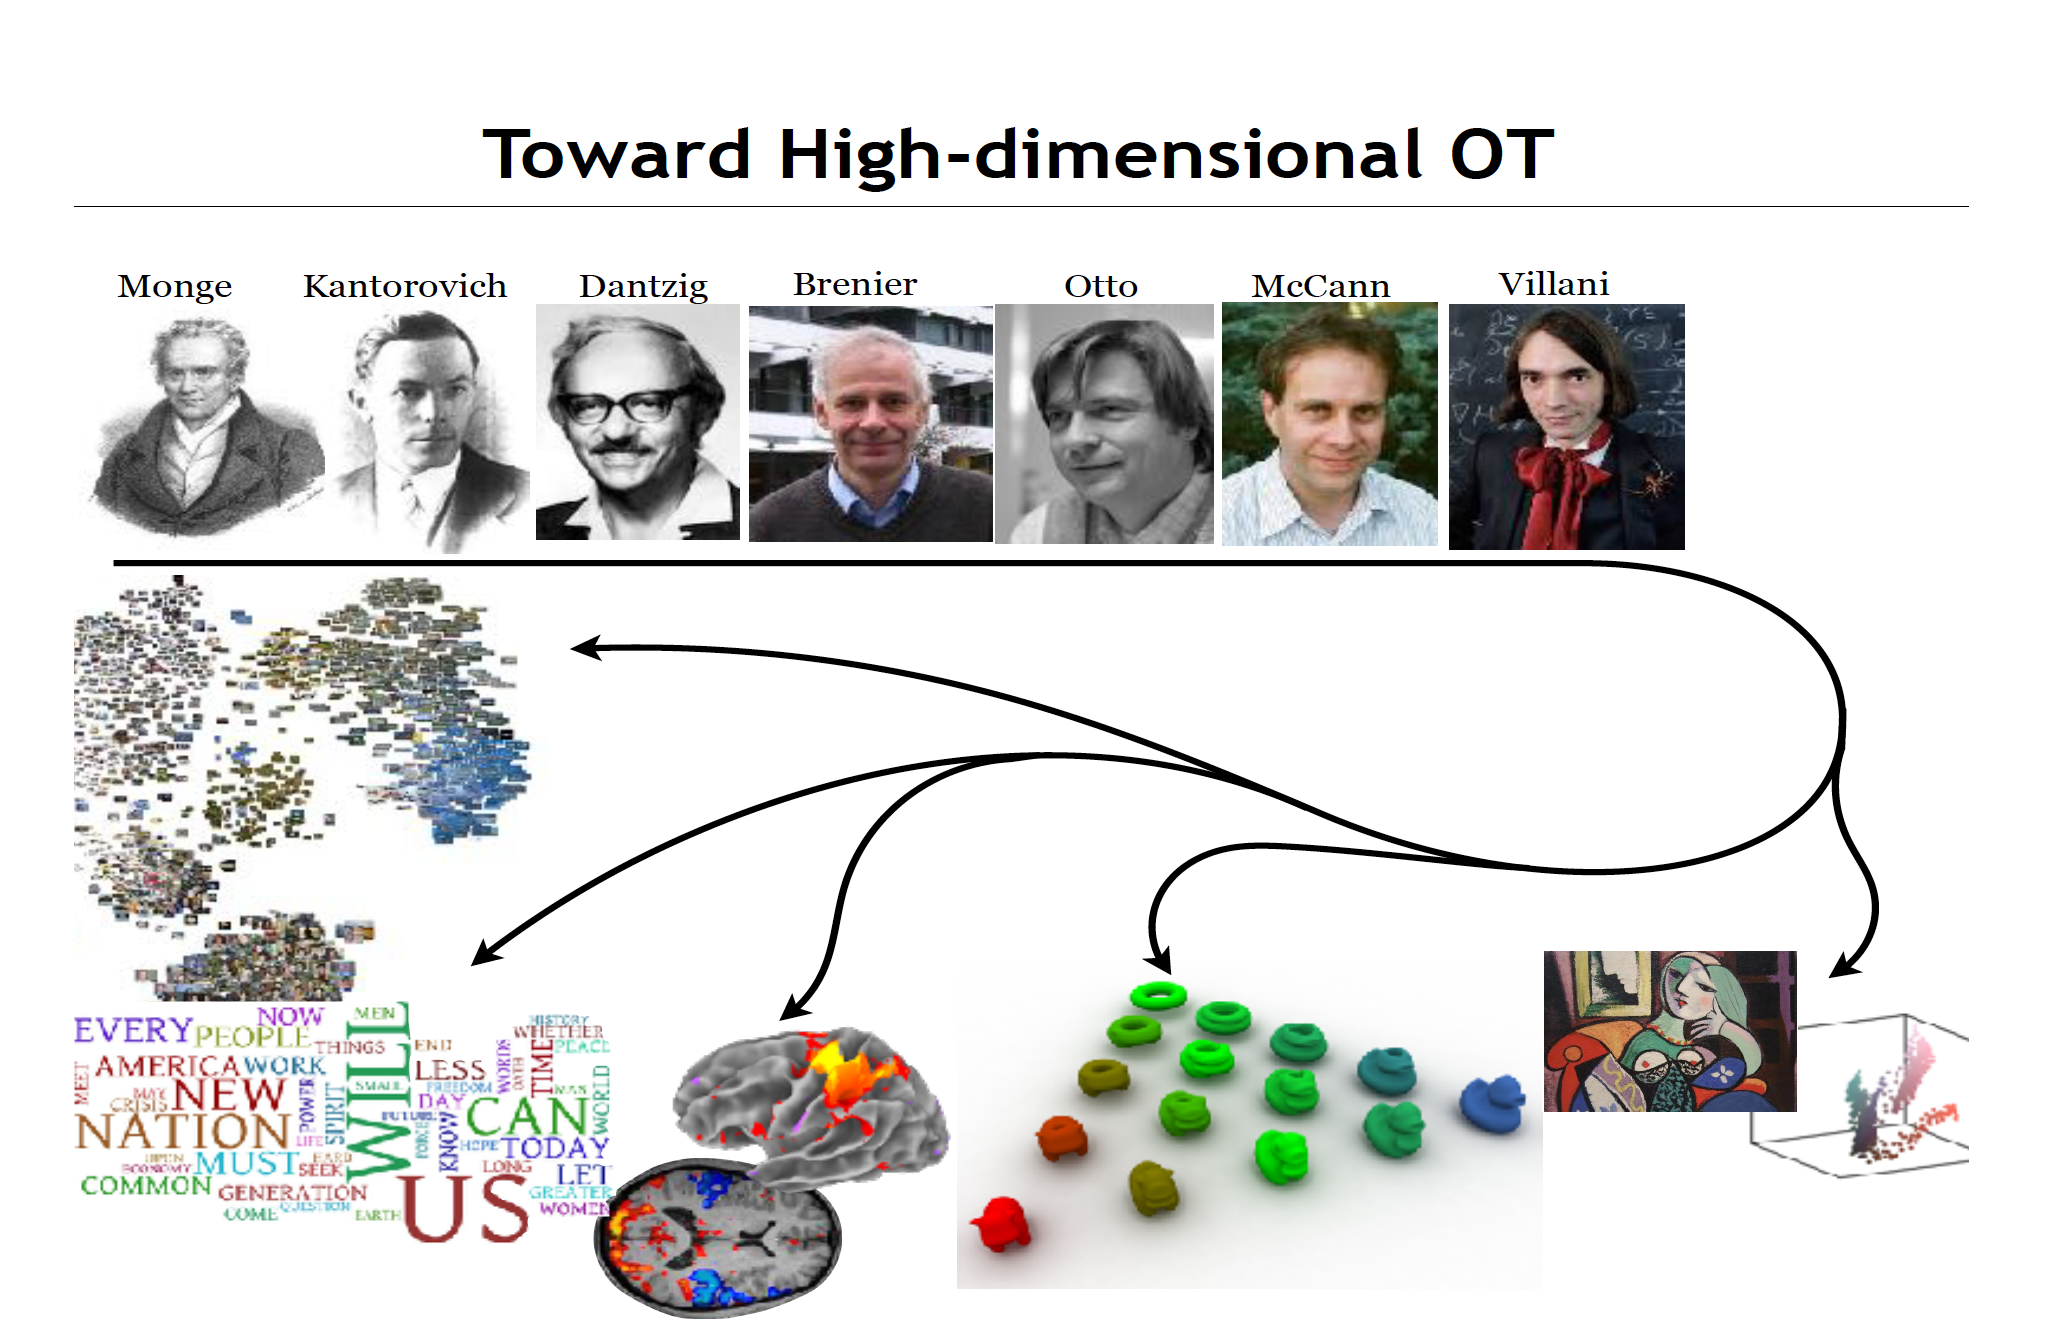
\includegraphics[width=0.6\linewidth]{history.png}}
        \end{figure}
\end{frame}

\begin{frame}{Optimal transport}
In recent years, optimal transport (a.k.a Earth mover's distance, Monge-Kantorovich problem, Wasserstein metric) has witnessed a lot of applications:
\vspace{0.5cm}
\begin{itemize} 
\item 1. Mean field games (Lions, Gangbo, Osher);
\item 2. Population Games via Fokker-Planck Equations (Li et.al. 2016, Degond et. al. 2014);
\item 3. Machine learning: Wasserstein Training of Boltzmann Machines (Cuturi et.al. 2015); Learning from Wasserstein Loss (Li et.al. 2018); Wasserstein GAN; Wasserstein statistics, and many more in NIPS 2015, 2016, 2017, 2018, 2019.
\end{itemize}
\end{frame}

\begin{frame}{Why optimal transport?}
Optimal transport provides a particular distance ($W$) among distributions, which relies on the distance on sample spaces $\Omega$
	\bequn
		\begin{aligned}
			W_p^p\lp \rho, \mu \rp & = \inf_{\pi \in \prod\lp \rho, \mu \rp} \int \lv x - y \rv^p d\pi\lp x, y \rp \ \text{(Wasserstein-p distance)}.
		\end{aligned}
	\eequn
Denote $X_0\sim \rho^0=\delta_{x_0}$, $X_1\sim \rho^1=\delta_{x_1}$. Compare
$$W_c(\rho^0,\rho^1)=\inf_{\pi\in\Pi(\rho^0, \rho^1)}\mathbb{E}_{(X_0, X_1)\sim\pi} c(X_0, X_1)=c(x_0,x_1);$$
Vs
$$\textrm{TV}(\rho^0,\rho^1)=\int_{\Omega}|\rho^0(x)-\rho^1(x)|dx=2;$$
Vs 
$$\textrm{KL}(\rho^0\|\rho^1)=\int_\Omega\rho^0(x)\log\frac{\rho^0(x)}{\rho^1(x)}dx=\infty.$$
\end{frame}

\begin{frame}{Dynamical formulation}
Wasserstein-2 distance has a dynamical formulation (Brenier et. al. 2000),
%\footnote{Benamou, Brenier, A computational fluid mechanics solution to the Monge-Kantorovich mass transfer problem, 2000.} 
namely it minimizes the kinetic energy of an evolution between $\mu$ and $\nu$:
\bequn
	\begin{aligned}
		W_2^2\lp \nu, \mu \rp & = \inf_{\rho_t}~\int_0^1 g_W(\partial_t\rho_t, \partial_t\rho_t)dt=\int_0^1\int_{\Omega} \nabla\Phi_t \cdot \nabla\Phi_t \rho_tdxdt,		\\
		& \ s.t. \ \rho_0 = \nu, \rho_1 = \mu,		\\
		& \qquad \p_t \rho_t + \nabla \cdot \lp \rho_t \nabla\Phi_t \rp = 0.
	\end{aligned}
\eequn
This dynamical formulation induces a metric structure on probability space (density manifold) $(\mathcal{P}(\Omega), g_W)$, which is an infinite-dimensional {\color{blue}Riemannian manifold}.
%\footnote{John D. Lafferty: The density manifold and configuration space quantization, 1988.} 
This requires to solve a PDE in high dimension while it has an explicit formula in 1-d sample space.
\end{frame}

\begin{frame}{Review of optimal transport on graph}
\JX{it is a bit controversial what is the audience for this content, it seems that for graph theorists, they do not totally agree with this.}
Although it had been deeply understood when sample spaces are Riemannian manifolds,
%\footnote{Otto, Generalization of an inequality by Talagrand and links with the logarithmic Sobolev inequality, 2000.} 
defining a canonical theory of Wasserstein geometry on graphs remains a question. 
\par
Several groups already establish some results on this direction:
\begin{itemize}
	\item 1. Heat flow on graph (Li et.al. 2017, 2018), under the choice of weight:
	\bequn	
		\begin{aligned}
			\nabla \Phi_{ij} & = \sqrt{w_{ij}}\lp \Phi_i - \Phi_j \rp,			\\
			\lp \nabla \cdot \lp \rho \nabla \Phi \rp \rp_i & = - \sum_{j \in N\lp i \rp} \sqrt{w_{ij}}\lp \Phi_i - \Phi_j \rp \lp \frac{\rho_i + \rho_j}{2} \rp.
		\end{aligned}
	\eequn
	\item 2. Geodesic in probability simplex. (W. Gangbo et. al. 2017)
	\item 3. Markov jump process as gradient flows. (J. Maas et. al. 2011, 2018)
\end{itemize}

\end{frame}

\begin{frame}{Gaussian mixture model (GMM)}
	Gaussian mixture models (GMM) are widely used in statistical inference 
	%\footnote{Huber, On Entropy Approximation for Gaussian Mixture Random Vectors, 2008} 
	(statistical models) and scientific computation.
	%\footnote{Jianfeng Lu, Numerical methods for stochastic differential equations based on Gaussian mixture, 2018}.
	\par
	A simple review of GMM:
	\bequn
	\begin{aligned}
	\rho: \Theta & \rightarrow \mcP\lp \mbR \rp, \quad \Theta \subset \mbR^{N - 1},			\\
	\theta & \mapsto \rho_{\theta} = \sum_{i = 1}^{N - 1} \theta_i \lp \rho_{i + 1} - \rho_i \rp + \rho_1 = \sum_{i = 1}^{N} p_i\rho_i, \\
	1  & = \theta_0 > \theta_1 > \cdots > \theta_{N - 1} > \theta_N = 0,			\\
	\rho_i & \sim \mcN\lp \mu_i, \sigma^2 \rp, \ \mu_1 < \mu_2 < \cdots < \mu_{N - 1} < \mu_N,
	\end{aligned}
	\eequn
	This work is based on the consideration of GMM.
\end{frame}

\begin{frame}{OT on GMM}
	Geometric structures on GMM:
	\begin{itemize}
		\item 1. Information geometry (Fisher-Rao metric): mixture family, mixture connection, duality, etc (N. Ay et. al., 2017).
		%\footnote{N. Ay, Information geometry, 2017}.
		\item 2. Wasserstein geometry: some researchers already consider optimal transport in GMM (Chen et. al. 2017).
		%\footnote{Yongxin Chen, Optimal transport for Gaussian mixture models, 2017} \footnote{Julie Delon, A Wasserstein-type distance in the space of Gaussian Mixture Models, 2019} 
		But they focus on the perspective of distance. \JX{need to mention the difference between our perspective, we focus on the metric while they 
		focus on the distance perspective. What is the key difference between metric and distance in one sentence? metric is infinitesimal distance}
	\end{itemize}
\end{frame}

\begin{frame}{Goals}
\vspace{0cm}
\begin{block}{Main Question:}
Is there a natural definition and a dynamical formulation of optimal transport on graphs or discrete spaces? What does the metric tensor look like in Gaussian mixture models? Can we use this to design numerical schemes?
\end{block}

\begin{block}{More related studies}
\begin{itemize} 
\item Wasserstein natural gradient (Li, Osher, Montufar et. al.)
\item Information geometry (S. Amari et. al.)
\item Gradient flows on graphs (J. Maas et. al.)
\item Wasserstein statistics (W. Li, J. Zhao et. al.)
\end{itemize}
\end{block}
\end{frame}

\begin{frame}{Scientific computing}
	\JX{This part is for audience of the scientific computing background, here we will mainly focus on the application in numerical PDE and 
	numerical analysis}
	Distance and geometric structure in probability space play important roles in scientific computation, both theoretic and computational:
	\vspace{5mm}
	\begin{itemize}
		\item 1. PDE %\footnote{Chow, Yat Tin, et al. "Algorithm for Hamilton–Jacobi equations in density space via a generalized Hopf formula." Journal of Scientific Computing 80.2 (2019): 1195-1239.} 
		and especially mean-field games (Osher, Gangbo, Li). 
		%\footnote{Ruthotto, Lars, et al. "A machine learning framework for solving high-dimensional mean field game and mean field control problems." Proceedings of the National Academy of Sciences 117.17 (2020): 9183-9193.}
		\item 2. Accelerated algorithms (Li et. al. 2019, 2020).
		%\footnote{Wuchen Li, Accelerated information flow, 2019.}
		\item 3. Deep learning approach in scientific computation (Osher et. al. 2020).
		%\footnote{Jason D. Lee, Optimal transport mapping via input convex neural networks.}
	\end{itemize}
\end{frame}

\begin{frame}{Our approach}
	We focus on the one-dimensional sample space to utilize the explicit formula for Wasserstein metric.
	\par
	\textbf{Step 1}: Define a (Fisher-Rao/Wasserstein) pull-back metric $G_W\lp \theta; \sigma \rp$ on GMMs, where $\theta$ is parameter and $\sigma$ is the variance.
	\begin{figure}[H]
          \centering
          \centerline{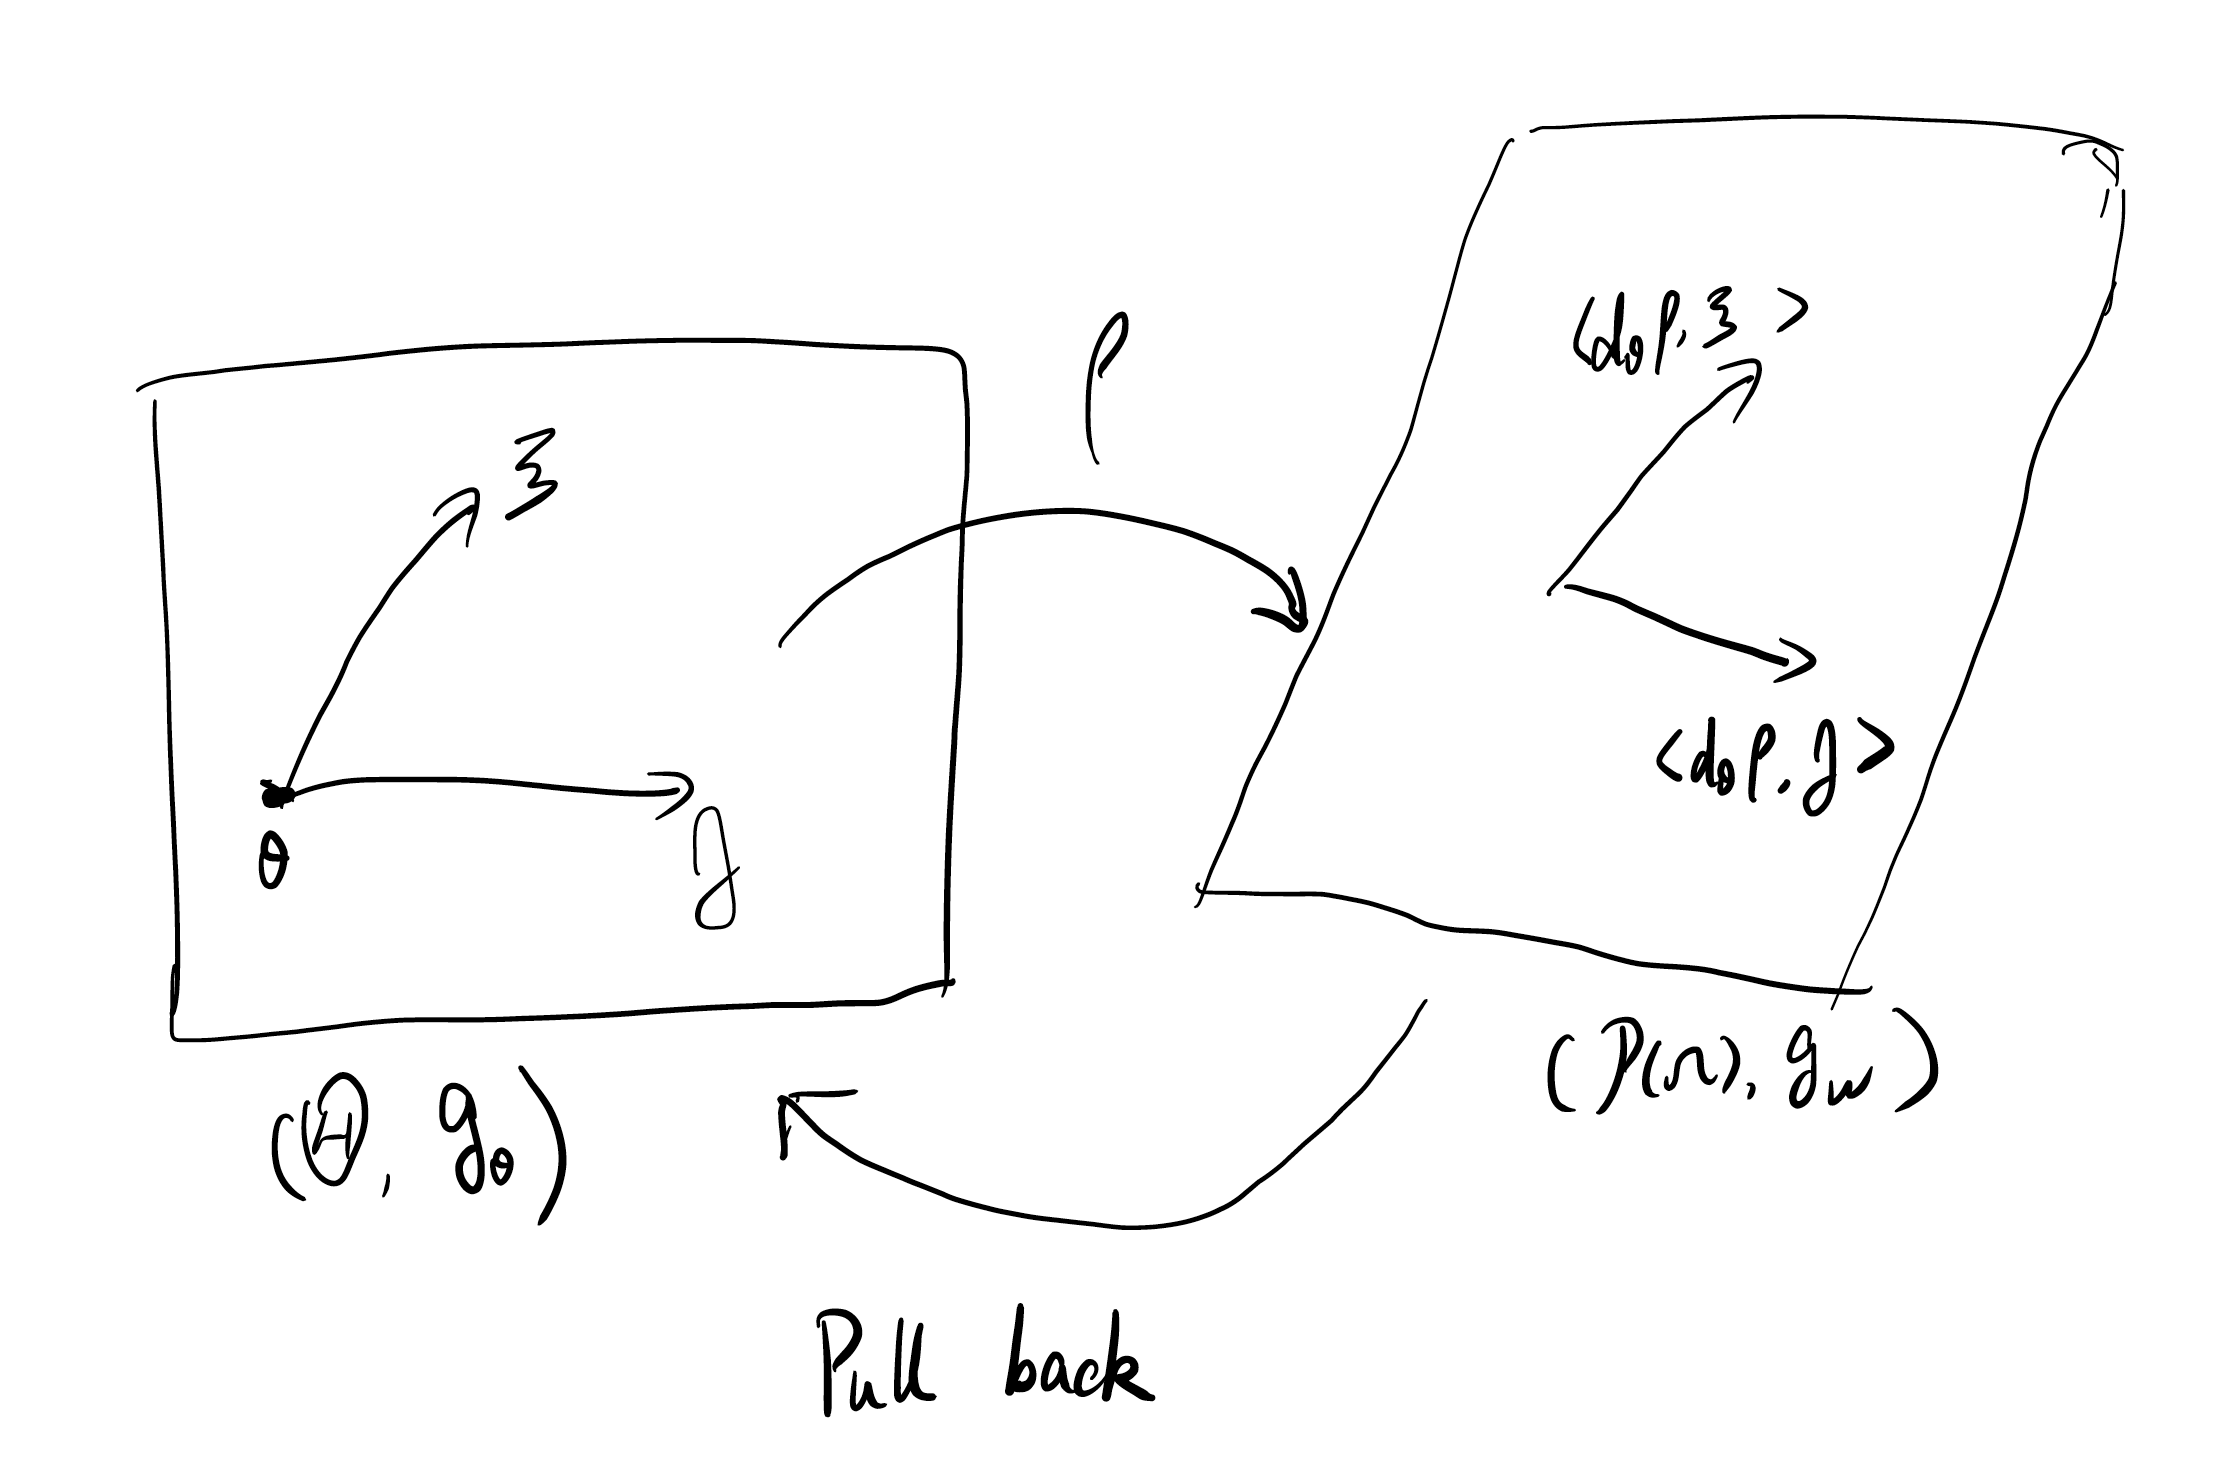
\includegraphics[width=0.7\linewidth]{pull_back.png}}
          \caption{Pull-back of the metric}
    	\end{figure}
\end{frame}

\begin{frame}{Our approach}
	\textbf{Step 2}: Rescale GMMs to approximate discrete spaces. As the variance of Gaussian tends to $0$, distributions weakly converge to a Dirac measure centered at its mean.
	\bequn
		\lim_{\sigma \rightarrow 0} \frac{G_W\lp \theta; \sigma \rp}{K\lp \sigma \rp} = G_{\wtd W}\lp \theta \rp.
	\eequn	
	\begin{figure}[H]
          \centering
          \centerline{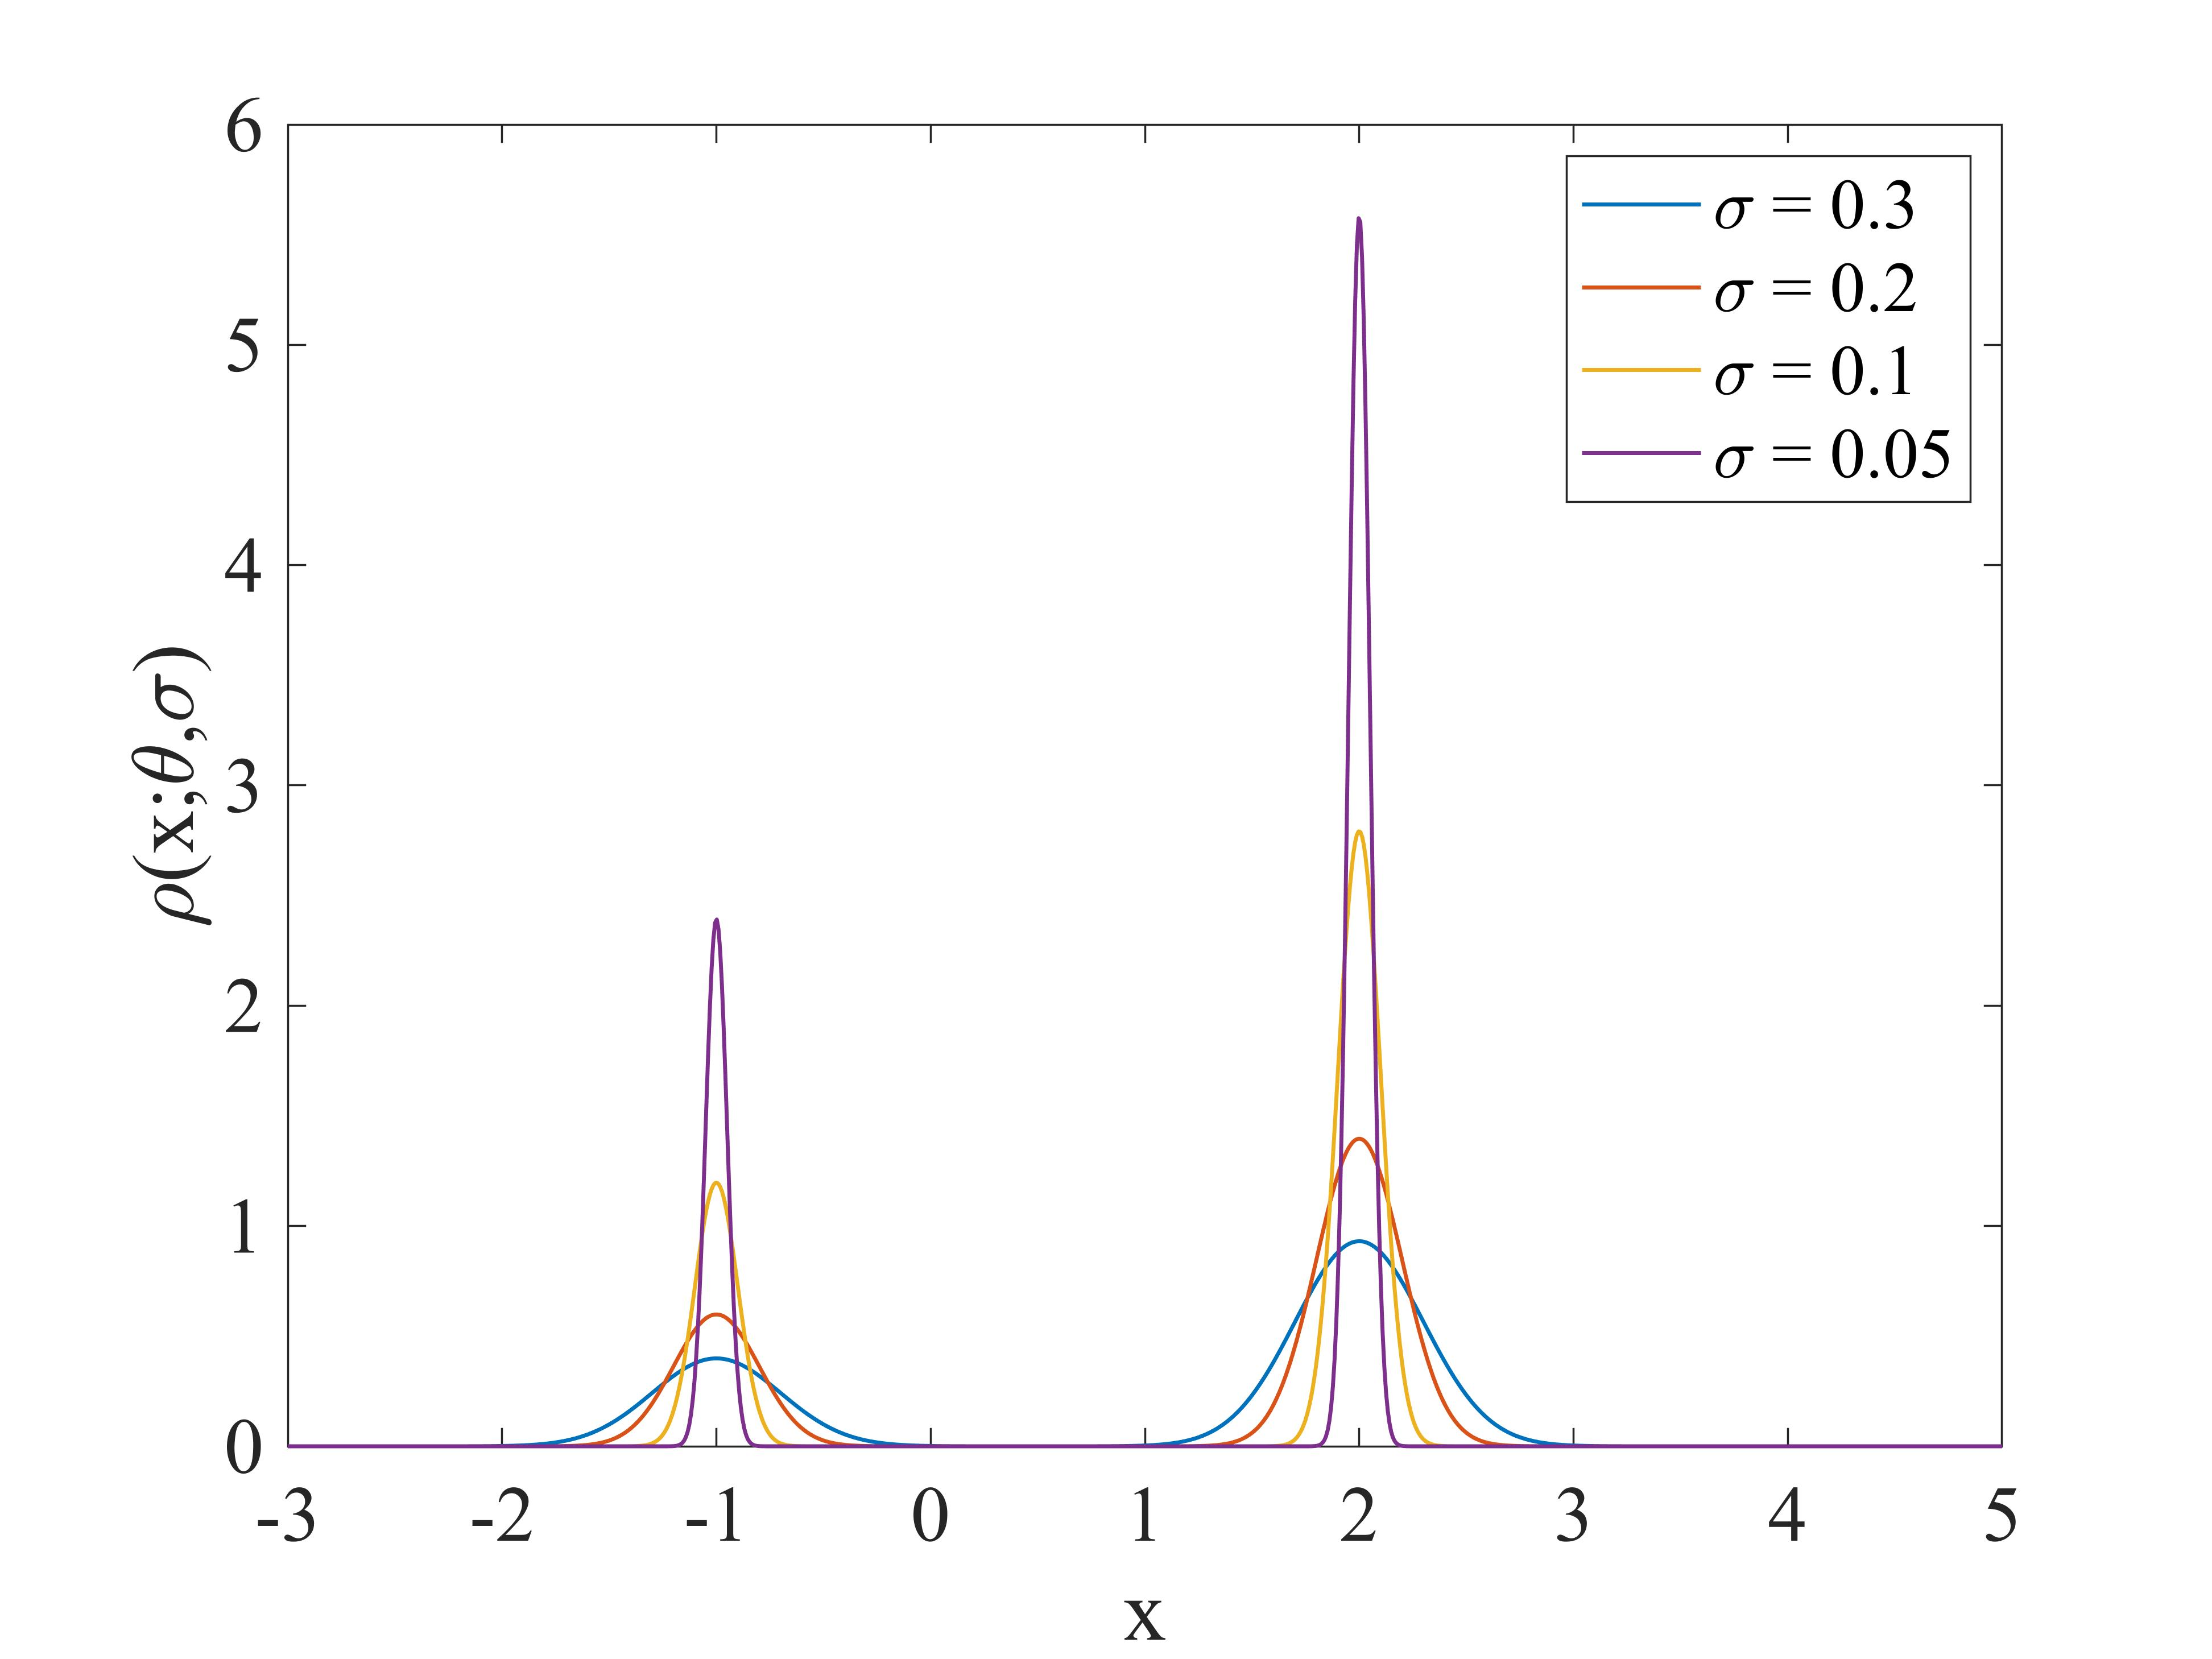
\includegraphics[width=0.55\linewidth]{Approx.jpg}}
          \caption{\scriptsize{The figure plots the density function of a family of Gaussian mixture given by $\rho\lp x \rp \sim 0.3 * \mcN\lp -1, \sigma \rp + 0.7 * \mcN\lp 2, \sigma \rp$.}}
    	\end{figure}
\end{frame}

\begin{frame}{Fisher-Rao pull-back metric on GMM}
\begin{example}
Explicit formula for Fisher-Rao metric in one-dimensional sample space reads
 \begin{equation*}
 g_F\lp \partial_i\rho(x;\theta), \partial_j\rho(x;\theta) \rp = G_F(\theta)_{ij}=\mathbb{E}_{\rho_\theta} \lp \frac{\frac{\partial}{\partial\theta_i}\rho(x;\theta)\frac{\partial}{\partial\theta_j}\rho(x;\theta)}{\rho(x;\theta)^2} \rp.
 \end{equation*}
In cases of GMM, it is given by
\bequn
 G_F(\theta)_{ij}=\mathbb{E}_{\rho_\theta} \lb \frac{\lp \rho_{i + 1}(x;\theta) - \rho_{i}(x;\theta) \rp\lp \rho_{j + 1}(x;\theta) - \rho_{j}(x;\theta) \rp}{\rho(x;\theta)^2} \rb,
\eequn
which can be simplified according to
\bequn
		\lim_{\sigma \rightarrow 0}\int \frac{\rho_i\lp x \rp \rho_j\lp x \rp}{\rho_{\theta}\lp x \rp}dx
			= \mbE_{x \sim \delta_{\mu_i}} \lim_{\sigma \rightarrow 0}\frac{\rho_j\lp x \rp}{\rho_{\theta}\lp x \rp}
			= \lim_{\sigma \rightarrow 0}\frac{\rho_j\lp \mu_i \rp}{\rho_{\theta}\lp \mu_i \rp} = \frac{\delta_{ij}}{p_i}.
	\eequn
\end{example}
\end{frame}

\begin{frame}{Scaling approximation Fisher-Rao metric}
	\begin{Thm}[Scaling Fisher-Rao metric]
	For a 1-d homogeneous GMM, the above scaling limit of Fisher information matrices is given by
	\scriptsize
	\bequn
		\begin{aligned}
		& \ G_{\wtd F}\lp \theta \rp 	\\
		= & \ \lim_{\sigma \rightarrow 0} G_F\lp \theta; \sigma \rp = \begin{pmatrix}
			\frac{1}{p_1} + \frac{1}{p_{2}} & - \frac{1}{p_2} & 0 & \cdots & 0 & 0 			\\
			- \frac{1}{p_2} & \frac{1}{p_2} + \frac{1}{p_{3}} & - \frac{1}{p_3} & \cdots & 0 & 0	\\
			0 & - \frac{1}{p_3} & \frac{1}{p_3} + \frac{1}{p_{4}} & \cdots & 0 & 0			\\
			\vdots & \vdots & \vdots & \ddots & \vdots & \vdots 						\\
			0 & 0 & 0 & \cdots & -\frac{1}{p_{N - 1}} & \frac{1}{p_{N - 1}} + \frac{1}{p_{N}}
		\end{pmatrix}.
		\end{aligned}
	\eequn
	\end{Thm}
	\normalsize
	\textbf{This coincides with original definition of Fisher-Rao metric on probability simplices!}
\end{frame}

\begin{frame}{Wasserstein pull-back metric on GMM}
\begin{example}
Explicit formula for Wasserstein metric in one-dimensional sample space reads
 \begin{equation*}
 G_W(\theta)_{ij}=\mathbb{E}_{\rho_\theta} \lp \frac{\frac{\partial}{\partial\theta_i}F(x;\theta)\frac{\partial}{\partial\theta_j}F(x;\theta)}{\rho(x;\theta)^2} \rp,
 \end{equation*}
where $F(x;\theta)$ is the cumulative distribution function of the density function $\rho(x;\theta)$. In case of GMM, it is given by
\bequn
 G_W(\theta)_{ij}=\mathbb{E}_{\rho_\theta} \lb \frac{\lp F_{i + 1}(x;\theta) - F_{i}(x;\theta) \rp\lp F_{j + 1}(x;\theta) - F_{j}(x;\theta) \rp}{\rho(x;\theta)^2} \rb,
\eequn
where $F_{i}(x;\theta)$ is the cumulative distribution function of the density function $\rho_i(x;\theta)$.
\end{example}
\end{frame}

\begin{frame}{Scaling approximation Wasserstein metric}
	\begin{Thm}[Scaling Wasserstein metric]
	For a 1-d homogeneous GMM with difference between adjacent components given by $d$, a scaling limit of Wasserstein information matrices is given by
	\scriptsize
	\bequn
		G_{\wtd W}\lp \theta \rp = \lim_{\sigma \rightarrow 0} \frac{G_W\lp \theta; \sigma \rp}{K\lp \sigma \rp} = \begin{pmatrix}
			\frac{1}{\sqrt{p_1p_{2}}} & 0 & 0 & \cdots & 0 & 0 			\\
			0 & \frac{1}{\sqrt{p_2p_{3}}} & 0 & \cdots & 0 & 0	\\
			0 & 0 & \frac{1}{\sqrt{p_3p_{4}}} & \cdots & 0 & 0			\\
			\vdots & \vdots & \vdots & \ddots & \vdots & \vdots 						\\
			0 & 0 & 0 & \cdots & 0 & \frac{1}{\sqrt{p_{N - 1}p_{N}}}
		\end{pmatrix}
	\eequn
	\normalsize
	The scaling factor appearing above is given by
	\bequn
		K\lp \sigma \rp = \sqrt{2\pi^3}\frac{\sigma^3}{d}e^{\half \lp \frac{d}{2\sigma}\rp^2}.
	\eequn
\end{Thm}
\end{frame}

\begin{frame}{Scaling approximation Wasserstein metric}
	Sketch of proof:
	\bequn
	\begin{aligned}
		\lp G_W\lp \theta \rp \rp_{i - 1, i - 1} & \ = \int \frac{\lp F_i - F_{i - 1} \rp^2}{\rho_{\theta}}dx \\
		& \ \stackrel{\Delta_1}{\Longrightarrow} \int_{\mu_{i - 1}}^{\mu_i} \frac{1}{p_{i - 1}\rho_{i - 1} + p_{i} \rho_i }dx \\
		& \ \stackrel{\Delta_2}{\Longrightarrow}  \text{Laplacian asymptotics}.
	\end{aligned}
	\eequn
	\begin{figure}[h]
  \centering
  \centerline{\includegraphics[width=0.52\linewidth]{decomp.jpg}}
  \caption{This figure plots an example of the function $\p_{\theta_i} F_{\theta}\lp x \rp$ for a GMM.}
\end{figure}
\end{frame}

\begin{frame}{$\Delta_1$ reduction}
	\JX{Yifan has remarked that maybe this can be understood from the perspective that the 
	discretized $\nabla \cdot (\rho \nabla)$ operator is a banded operator.}
\end{frame}

\begin{frame}{$\Delta_2$ reduction}
	A complicated version of Laplacian integral.
\end{frame}

\begin{frame}{Scaling approximation Wasserstein metric}
	\JX{A good point after introduce this metric is to discuss its properties etc.}
	This scaling approximate metric is natural in the following senses:
	\begin{itemize}
		\item 1. In Fisher-Rao case, this scaling approximate metric coincides with original definition.
		\item 2. It can be derived as the scaling approximate of many general mixture models (Laplacian mixture models). Intuitively, it is the scaling approximation of most mixture models whose components decay exponentially or in other word, obey some concentration inequalities.
		\item 3. It is natural in the sense of gradient flow.
	\end{itemize}
\end{frame}

\begin{frame}{Inhomogeneous GMM}
	What if the gap between adjacent components are not the same? $\mu_{i + 1} - \mu_i \neq \mu_{j + 1} - \mu_j$
	\begin{itemize}
		\item Homogeneous lattice $\Longleftrightarrow$ GMM with same variances for components.
		\item Inhomogeneous lattice $\Longleftrightarrow$ GMM with different variances for components.
	\end{itemize}
	\begin{Thm}[informal]
	For a 1-d inhomogeneous GMM with difference between adjacent components given by $\mu_{i + 1} - \mu_i = d_i$, choose the variances of components as $\sigma_i = s_i \sigma$ such that the condition below is satisfied
	\bequ\label{var-cond}
		\frac{d_1}{s_1 + s_2}  = \frac{d_2}{s_2 + s_3} = \cdots = \frac{d_{N - 1}}{s_{N - 1} + s_N} = d.
	\eequ
	 A scaling limit of Wasserstein information matrices is again diagonal.
\end{Thm}
\end{frame}

\begin{frame}{Extended GMM}

	Now, we discuss an extended GMM, which is able to be tackled in our framework. Recall GMMs as:
	\bequn
	\begin{aligned}
		\rho_{\theta} = \sum_{i = 1}^{N - 1} \theta_i \lp \rho_{i + 1} - \rho_i \rp + \rho_1, \qquad \theta_{i - 1} \geq 	\theta_i \geq 0, \quad & \forall i = 2,...,N,		\\
		\rho_i \sim \mcN\lp \mu_i, \sigma \rp, \quad & \forall i = 1,...,N.
	\end{aligned}
	\eequn
	\par
	In ordinary GMMs, the $\mu_i$s are constants while only $\theta_i$s are parameters. In extended GMMs, both these two sets are parameters, namely, the means of each components can vary.
\end{frame}

\begin{frame}{Extended GMMs and Wasserstein information geometry}	
	\small
	\begin{Thm}[Wasserstein information geometry of extended GMMs] 
	For the extended GMM, we have the following relationship between the Wasserstein information matrix(WIM) of the set of tangent vectors $\frac{\p}{\p \mu_i}$s and Fisher information matrix(FIM) of the set of tangent vectors $\frac{\p}{\p \theta_i}$s
	\bequn\label{WIG-eq1}
		G_F = \Sigma G_W \Sigma^T,
	\eequn
	where $\lp G_F \rp_{ij} = g_F\lp \frac{\p}{\p \theta_i}, \frac{\p}{\p \theta_j} \rp$, $\lp G_W \rp_{ij} = g_W\lp \frac{\p}{\p \mu_i}, \frac{\p}{\p \mu_j} \rp$ and the matrix $\Sigma \in \mbR^{N-1,N}$ appears above is given by
	\scriptsize
	\bequn
		\Sigma = \begin{pmatrix}
			- \frac{1}{p_1} & \frac{1}{p_2} & 0 & \cdots & 0 & 0		\\
			0 & - \frac{1}{p_2} & \frac{1}{p_2} & \cdots & 0	& 0		\\
			\vdots & \vdots & \ddots & \cdots	& \cdots & \cdots				\\
			0 & 0 & \cdots & - \frac{1}{p_{N - 2}} & \frac{1}{p_{N - 1}} & 0		\\
			0 & 0 & 0 & \cdots & - \frac{1}{p_{N - 1}} & \frac{1}{p_N}
		\end{pmatrix}.
	\eequn 
\end{Thm}
\end{frame}

\begin{frame}{Extended GMMs and Wasserstein information geometry}	
	This result on the connection between Wasserstein information matrix and Fisher information matrix could be understood simply using the language of score functions.
	\par
	Since WIM and FIM play essential roles in statistical theory (Li et. al. 2019),
	%\footnote{Wuchen Li, Wasserstein information matrix, 2019}
	 it will be interesting to find statistical illustrations and corollaries of this result.
\end{frame}

\begin{frame}{Scaling approximation Wasserstein metric}
	\begin{Thm}[Scaling Wasserstein metric for extended GMMs]
	The Wasserstein metric in 1-d extended homogeneous GMM is given by following in block form
	\small
	\bequn
		\begin{aligned}
			& \lim_{\sigma \rightarrow 0}G_{W}^{(ext)}\lp \theta, \mu; \sigma \rp = \begin{pmatrix}
				\lp G_{\wtd W}^{(ext)} \rp_{\theta\theta} & \lp G_{\wtd W}^{(ext)} \rp_{\theta\mu}		\\
				\lp G_{\wtd W}^{(ext)} \rp_{\mu\theta} & \lp G_{\wtd W}^{(ext)} \rp_{\mu\mu}
			\end{pmatrix},						\\
			& \lp G_{\wtd W}^{(ext)} \rp_{\theta\theta} = K\lp \sigma \rp \begin{pmatrix}
				\frac{1}{\sqrt{p_1p_2}} & 0 & \cdots & 0		\\
				0 & \frac{1}{\sqrt{p_2p_3}} & \cdots & 0		\\
				\vdots & \vdots & \ddots & \vdots \\
				0 & 0 & \cdots & \frac{1}{\sqrt{p_{N - 1}p_N}}
			\end{pmatrix}, \\
			& \lp G_{\wtd W}^{(ext)} \rp_{\mu\mu} = \begin{pmatrix}
				p_{1} & 0 & \cdots & 0		\\
				0 & p_{2} & \cdots & 0		\\
				\vdots & \vdots & \ddots & \vdots \\
				0 & 0 & \cdots & p_{N}
			\end{pmatrix}.
		\end{aligned}
	\eequn
\end{Thm}
\end{frame}

\begin{frame}{Scaling approximation Wasserstein metric}
	\small
	\begin{Thm}[Scaling Wasserstein metric for extended GMMs]
		\bequn
			\begin{aligned}
			& \ \lp \lp G_{\wtd W}^{(ext)} \rp_{\mu\theta} \rp^T \\
			= & \  \lp G_{\wtd W}^{(ext)} \rp_{\theta\mu} = \begin{pmatrix}
				\frac{\mu_2 - \mu_1}{2} & \frac{\mu_2 - \mu_1}{2} & 0 & \cdots & 0 & 0		\\
				0 & \frac{\mu_3 - \mu_2}{2} & \frac{\mu_3 - \mu_2}{2} & \cdots & 0 & 0		\\
				\vdots & \vdots & \vdots & \ddots & \vdots & \vdots \\
				0 & 0 & 0 & \cdots & \frac{\mu_{N - 1} - \mu_{N - 2}}{2} & 0		\\
				0 & 0 & 0 & \cdots & \frac{\mu_N - \mu_{N - 1}}{2} & \frac{\mu_N - \mu_{N - 1}}{2}
			\end{pmatrix}.	
			\end{aligned}
		\eequn
	\end{Thm}
	\normalsize
	Due to the existence of factor $K\lp \sigma \rp$, the scaling metric tensor has a multi-scale phenomenon, i.e. its block form has different orders in different blocks. This properties will the reason for multi-scale phenomenons in gradient flows.
\end{frame}

\begin{frame}{Parametric gradient flows}	
	Given a function $\mcE\lp \theta \rp$ on a parametric space $\Theta$ with metric given by $G\lp \theta \rp$, we define the gradient flow associated with this function as
	\bequn
		\dot{\theta} = - G\lp \theta \rp^{-1} \nabla_{\theta} \mcE\lp \theta \rp,
	\eequn
	where $\nabla_{\theta} \mcE\lp \theta \rp$ is ordinary Euclidean gradient. Since in GMM, parameters $\theta_i$s do not carry any physical meaning, we write the gradient flows equations for parameters $p_i$s
	\bequn
		\dot{p}_i = \dot{\theta}_{i - 1} - \dot{\theta}_i = \lp G\lp \theta \rp^{-1} \nabla_{\theta} \mcE\lp \theta \rp \rp_{i} - \lp G\lp \theta \rp^{-1} \nabla_{\theta} \mcE\lp \theta \rp \rp_{i - 1}.
	\eequn
\end{frame}

\begin{frame}{Gradient flows in scaling Wasserstein geometry}	
	Following the discussion in Villani,
	%\footnote{Villani, Topics in optimal transport, 2003}, 
	we derive the gradient flow equations of potential, internal, and interaction energy functional on density manifold and scaling Wasserstein geometry
	\bequn
	\begin{aligned}
		\textbf{internal energy:} & \qquad \mcU\lp \rho \rp = \int U\lp \rho\lp x \rp \rp dx = \sum_{i = 1}^N U\lp p_i \rp,		\\
		\textbf{potential energy:} & \qquad \ \mcV\lp \rho \rp = \int V\lp x \rp d\rho = \sum_{i = 1}^N V_i p_i, 	\\
		\textbf{interaction energy:} & \qquad \mcW\lp \rho \rp = \half \int\int W\lp x - y \rp \rho\lp x \rp\rho \lp y \rp dxdy \\
		& \qquad \qquad \ \  = \half\sum_{i, j = 1}^N W_{ij} p_i p_j.		\\
	\end{aligned}
	\eequn	
\end{frame}

\begin{frame}{Gradient flows in scaling Wasserstein geometry}
	We first show the continuous gradient flow on density manifold:
	\bequn
	\begin{aligned}
		\textbf{internal energy:} & \quad \p_t \rho = - \nabla \cdot \lp \rho \nabla U'\lp \rho \rp \rp,		\\
		\textbf{potential energy:} & \quad \p_t \rho = - \nabla \cdot \lp \rho \nabla V \rp,	\\
		\textbf{interaction energy:} & \quad \p_t \rho = - \nabla \cdot \lp \rho \nabla \lp W * \rho \rp \rp.		\\
	\end{aligned}
\eequn
	These are well-known facts in the community of optimal transport.
\end{frame}

\begin{frame}{Gradient flows in scaling Wasserstein geometry}
	\small
	\bequn
	\begin{aligned}
		\textbf{internal energy:} & \quad \dot{p_i} = - \sqrt{p_i p_{i - 1} } \lp U'\lp p_i \rp - U'\lp p_{i - 1} \rp \rp \\
		& \qquad \quad   + \sqrt{p_i p_{i + 1} } \lp U'\lp p_{i + 1} \rp - U'\lp p_{i} \rp \rp,		\\
		\textbf{potential energy:} & \quad \dot{p_i} = - \sqrt{p_i p_{i - 1} } \lp V_i - V_{i - 1} \rp + \sqrt{p_i p_{i + 1} } \lp V_{i + 1} - V_{i} \rp,	\\
		\textbf{interaction energy:} & \quad \dot{p_i} = - \sqrt{p_i p_{i - 1} } \lp \sum_{k = 1}^N W_{ik}p_k - \sum_{k = 1}^N W_{i-1, k}p_k \rp \\
		& \qquad \quad + \sqrt{p_i p_{i + 1} } \lp \sum_{k = 1}^N W_{i + 1, k}p_k - \sum_{k = 1}^N W_{ik}p_k \rp.		\\
	\end{aligned}
\eequn
	\normalsize
	\par
	We prove the consistency of these numerical discretization, i.e. they converge to their continuous counterpart.
\end{frame}

\begin{frame}{Properties of gradient flows}	
	We establish the following properties for this parametric gradient flows:
	\begin{itemize}
		\item 1. positivity
		\item 2. conservation of mass
		\item 3. long time existence
		\item 4. consistency
	\end{itemize}
\end{frame}

\begin{frame}{Gradient flows in extended GMM}	
	Based on the scaling metric for extended GMM, we derive following gradient flow equation.
	\small
	\begin{Thm}[Gradient flow in extended GMM]\label{ext-general-thm}
	The gradient flow w.r.t. a potential energy functional $($interaction energy functionals$)$ $\mcE\lp \rho \rp = \sum_{i = 1}^N p_i V\lp \mu_i \rp$ $(\mcE\lp \rho \rp = \sum_{1 \leq i < j \leq N} p_i p_j W\lp \lv \mu_i - \mu_j \rv \rp)$ is provided below
	\tiny
	\bequn\label{ext-general}
		\begin{aligned}
			\dot{\theta}_i = & \ - \frac{\sqrt{p_ip_{i + 1}}}{K\lp \sigma \rp}\lp \p_{\theta_i} \mcE\lp \rho \rp - \frac{\mu_{i + 1} - \mu_i}{2}\lp  \frac{\p_{\mu_i} \mcE\lp \rho \rp}{p_i} + \frac{\p_{\mu_{i + 1}} \mcE\lp \rho \rp}{p_{i + 1}} \rp \rp, \quad i = 1,2, \cdots, N - 1,	\\
			\dot{\mu}_i = & \ - \frac{1}{p_i}\p_{\mu_i} \mcE\lp \rho \rp + \frac{1}{K\lp \sigma \rp}\lp \sqrt{\frac{p_{i + 1}}{p_{i}}}\frac{\mu_{i + 1} - \mu_i}{2}\p_{\theta_i} \mcE\lp \rho \rp + \sqrt{\frac{p_{i - 1}}{p_{i}}}\frac{\mu_{i} - \mu_{i - 1}}{2}\p_{\theta_{i - 1}} \mcE\lp \rho \rp \rp, \\
			& \ \quad i = 2, 3,\cdots, N - 1,
		\end{aligned}
	\eequn
	\small
	where we ignore the equation for end-point parameters $\mu_1, \mu_N$ since they are not consistent with this framework.
\end{Thm}
	
\end{frame}

\begin{frame}{Analysis of gradient flows in extended GMMs}
	There are following interesting aspects in above gradient flow equations:
	\begin{itemize}
		\item 1. The flows of means parameters $\mu_i$s and ratio parameters $p_i$s have different orders. Hence they converge to equilibrium in different time scales.
		\item 2. The flow equations of parameters $\mu_i$ have two terms of different orders.
		\item 3. Comparing the flow equations of parameters $p_i$s with previous flows equations, we find an extra term.
	\end{itemize}
\end{frame}

\begin{frame}{Numerical experiments}
	\small
	\bequn
	\dot{p}_{i} = - \frac{1}{d^2} \lp \sqrt{p_{i - 1}p_i}\log \frac{p_i}{p_{i - 1}} - \sqrt{p_{i + 1}p_i}\log \frac{p_{i + 1}}{p_{i}} \rp,
\eequn
where $p_i$ is the mass on i-th lattice and $d$ is the gap, $\Delta t$ is the stepsize.
\begin{figure}[h]
  \centering
  \centerline{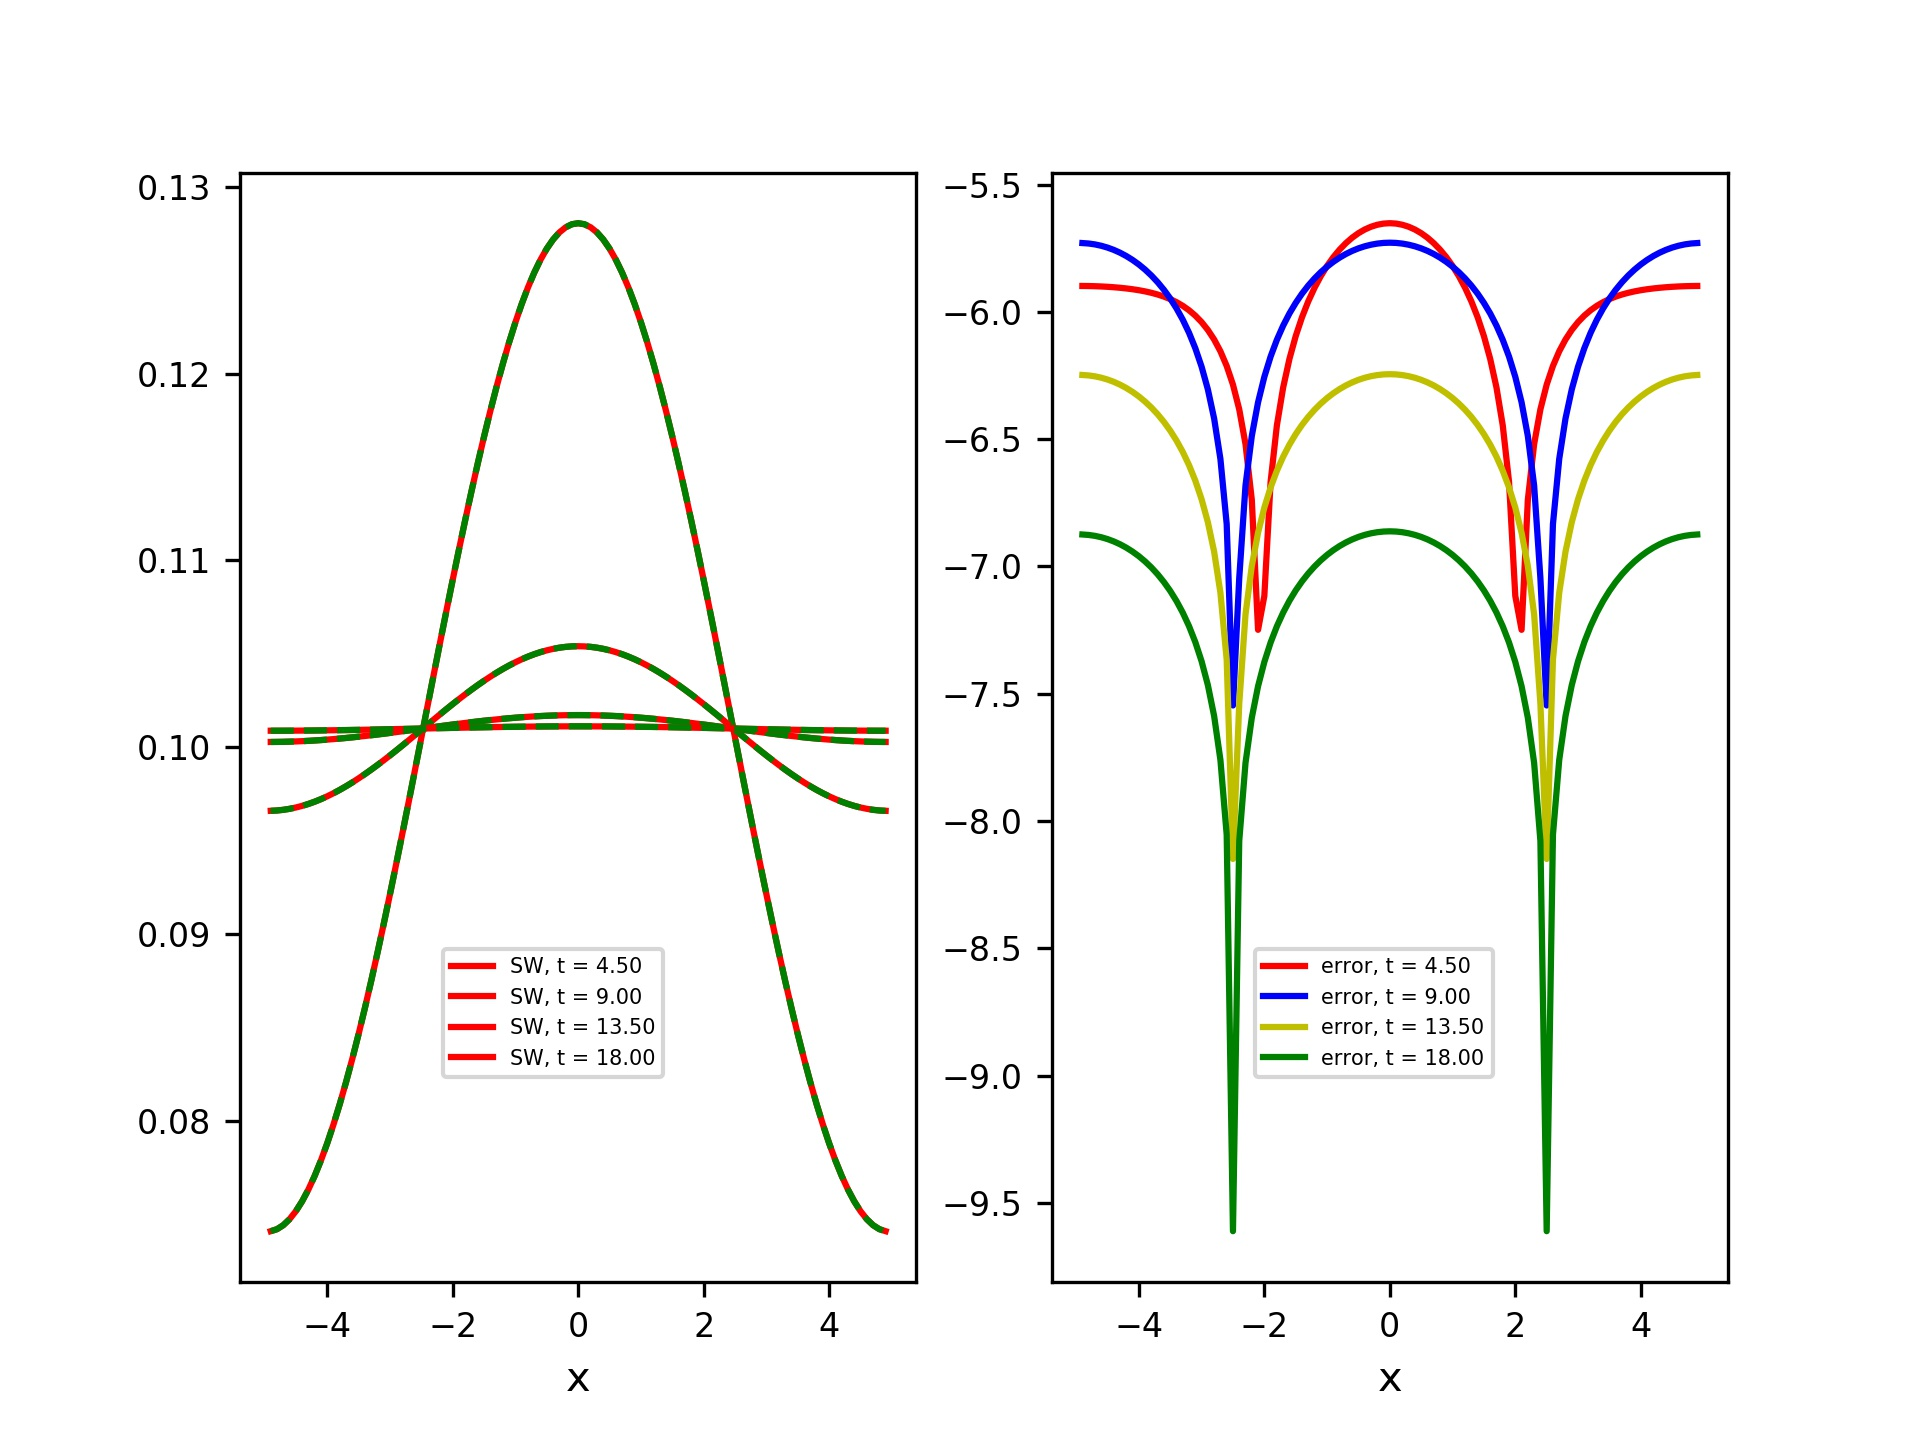
\includegraphics[width=0.75\linewidth]{heat1D.jpg}}
  \caption{\scriptsize{This figure plots a simulation of the 1-d heat flow via the discretization introduced in this paper. The gap of the lattice is set as $d = 0.01$. And the time step is set as $\Delta t = 0.000005$. The initial distribution is given by $\rho\lp x; 0 \rp = \mathbf{1}_{[-0.5, 0.5]}\lp x \rp$ and we consider its restriction to the interval $[-1, 1]$.}}
\end{figure}
\end{frame}

\begin{frame}{Numerical experiments}
\scriptsize
	\bequn
	\begin{aligned}
	\dot{p}_{ij} = & \ - \frac{1}{d^2} \lp \sqrt{p_{i - 1,j}p_{ij}}\log \frac{p_{ij}}{p_{i - 1,j}} - \sqrt{p_{i + 1,j}p_{ij}}\log \frac{p_{i + 1,j}}{p_{ij}} \rpt			\\
	& \ \left. \qquad + \sqrt{p_{i,j - 1}p_{ij}}\log \frac{p_{ij}}{p_{i,j - 1}} - \sqrt{p_{i,j + 1}p_{ij}}\log \frac{p_{i,j + 1}}{p_{ij}} \rp.
	\end{aligned}
\eequn
\begin{figure}[h]
  \centering
  \centerline{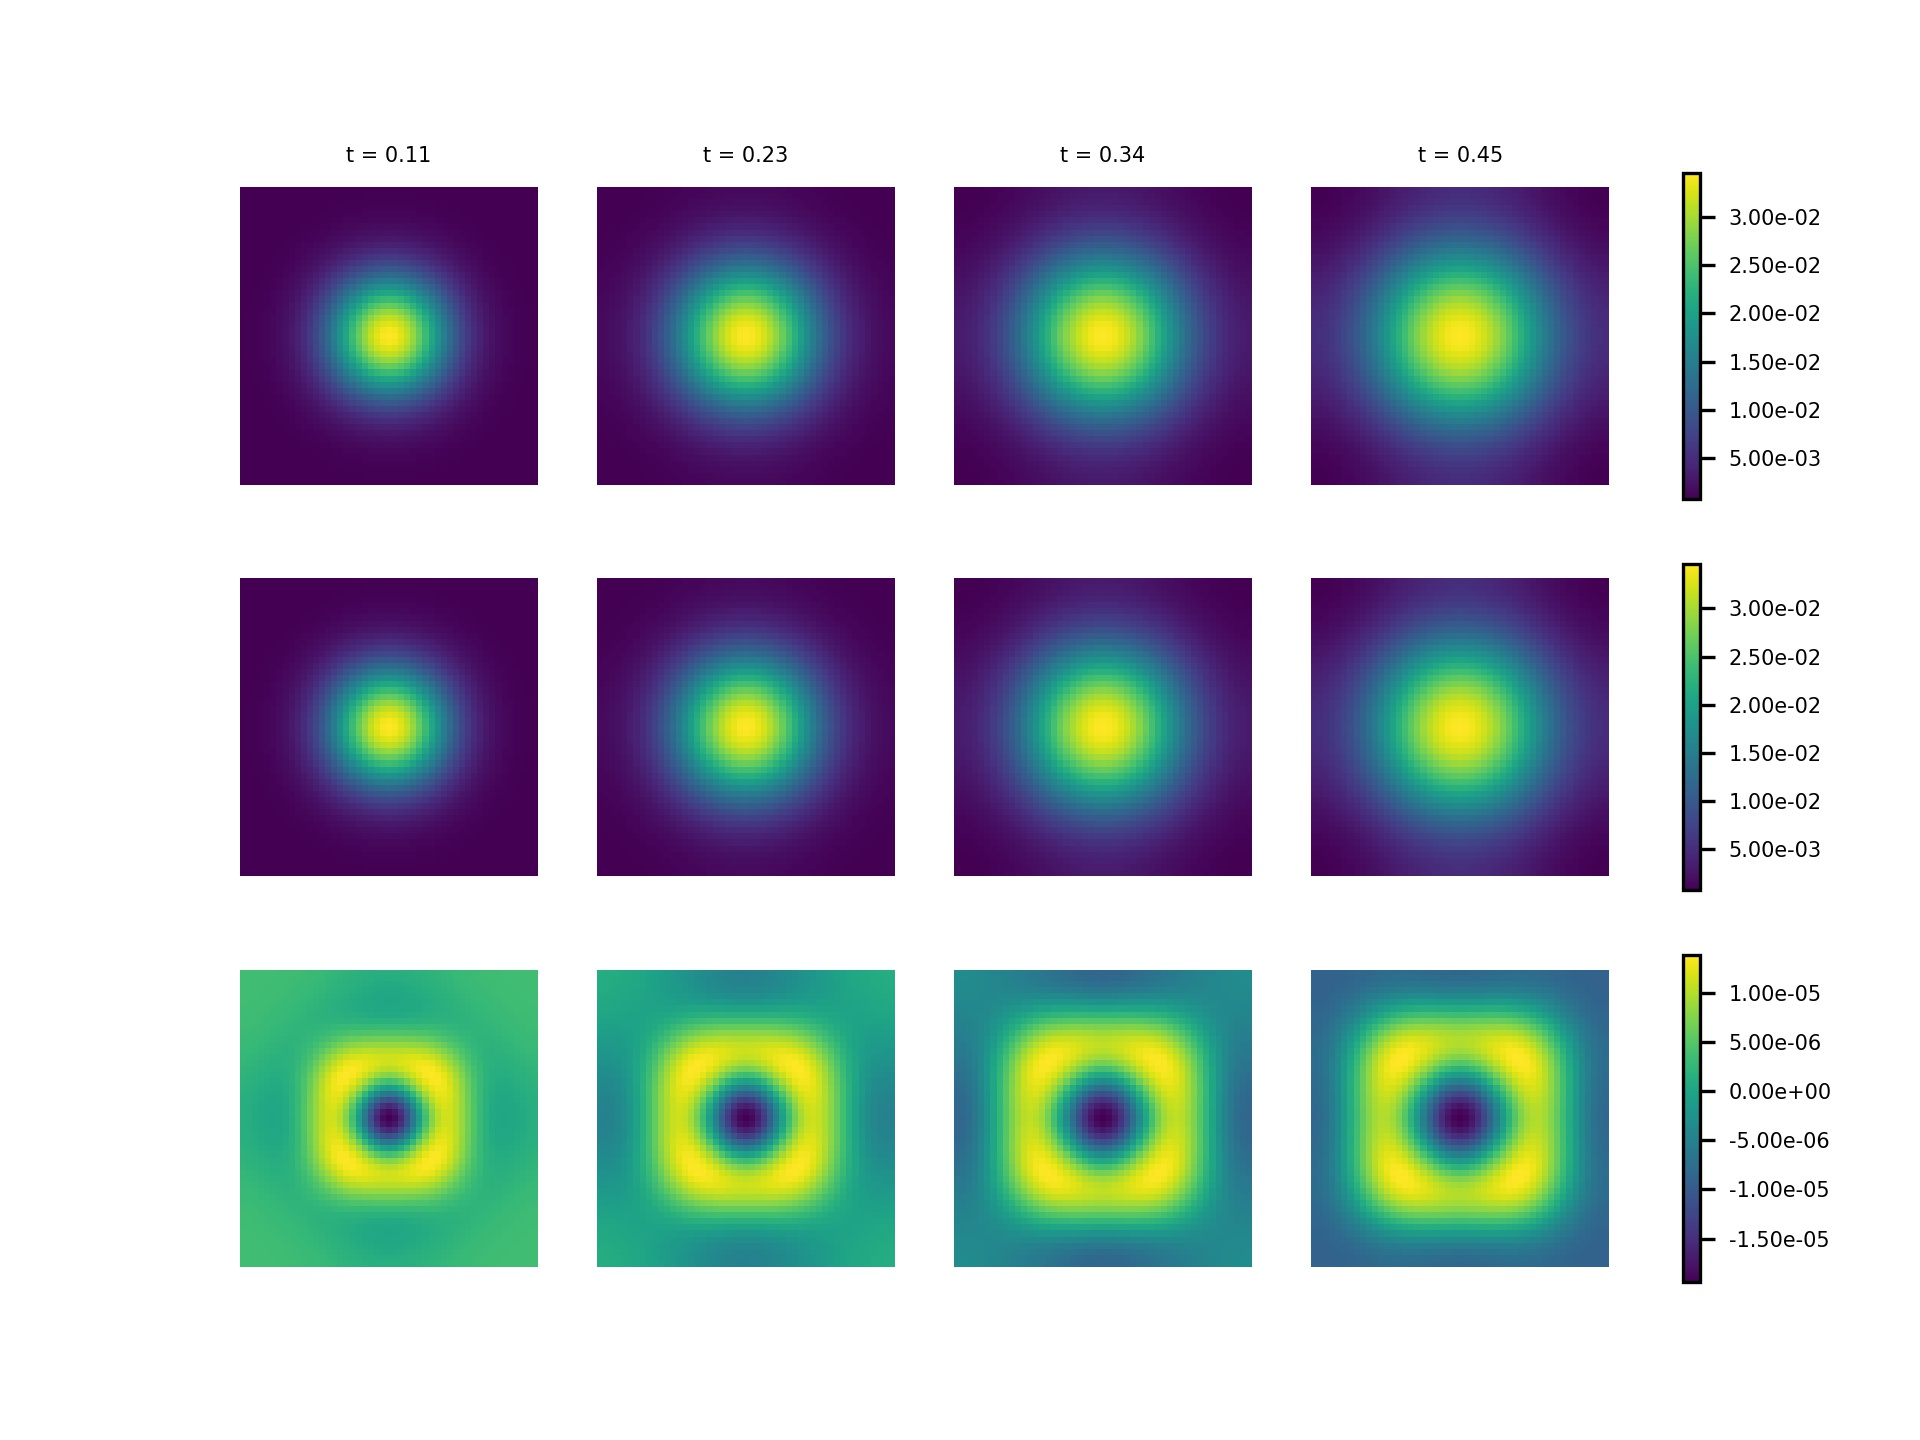
\includegraphics[width=0.7\linewidth]{heat2D.jpg}}
  \caption{\scriptsize{Simulation of a 2-d heat flow via discretization in this paper. The gap of the lattice and the time step are set as $d = 0.01, \Delta t = 2.5 \times 10^{-6}$ respectively. The initial distribution is given by $\rho\lp \mfx; 0 \rp = \mathbf{1}_{[-0.5, 0.5] \times [-0.5, 0.5]}\lp \mfx \rp$ and we consider its restriction to the interval $[-1, 1] \times [-1, 1]$.}}
\end{figure}
\end{frame}

\begin{frame}{Numerical experiments}
\begin{figure}[h]
  \centering
  \centerline{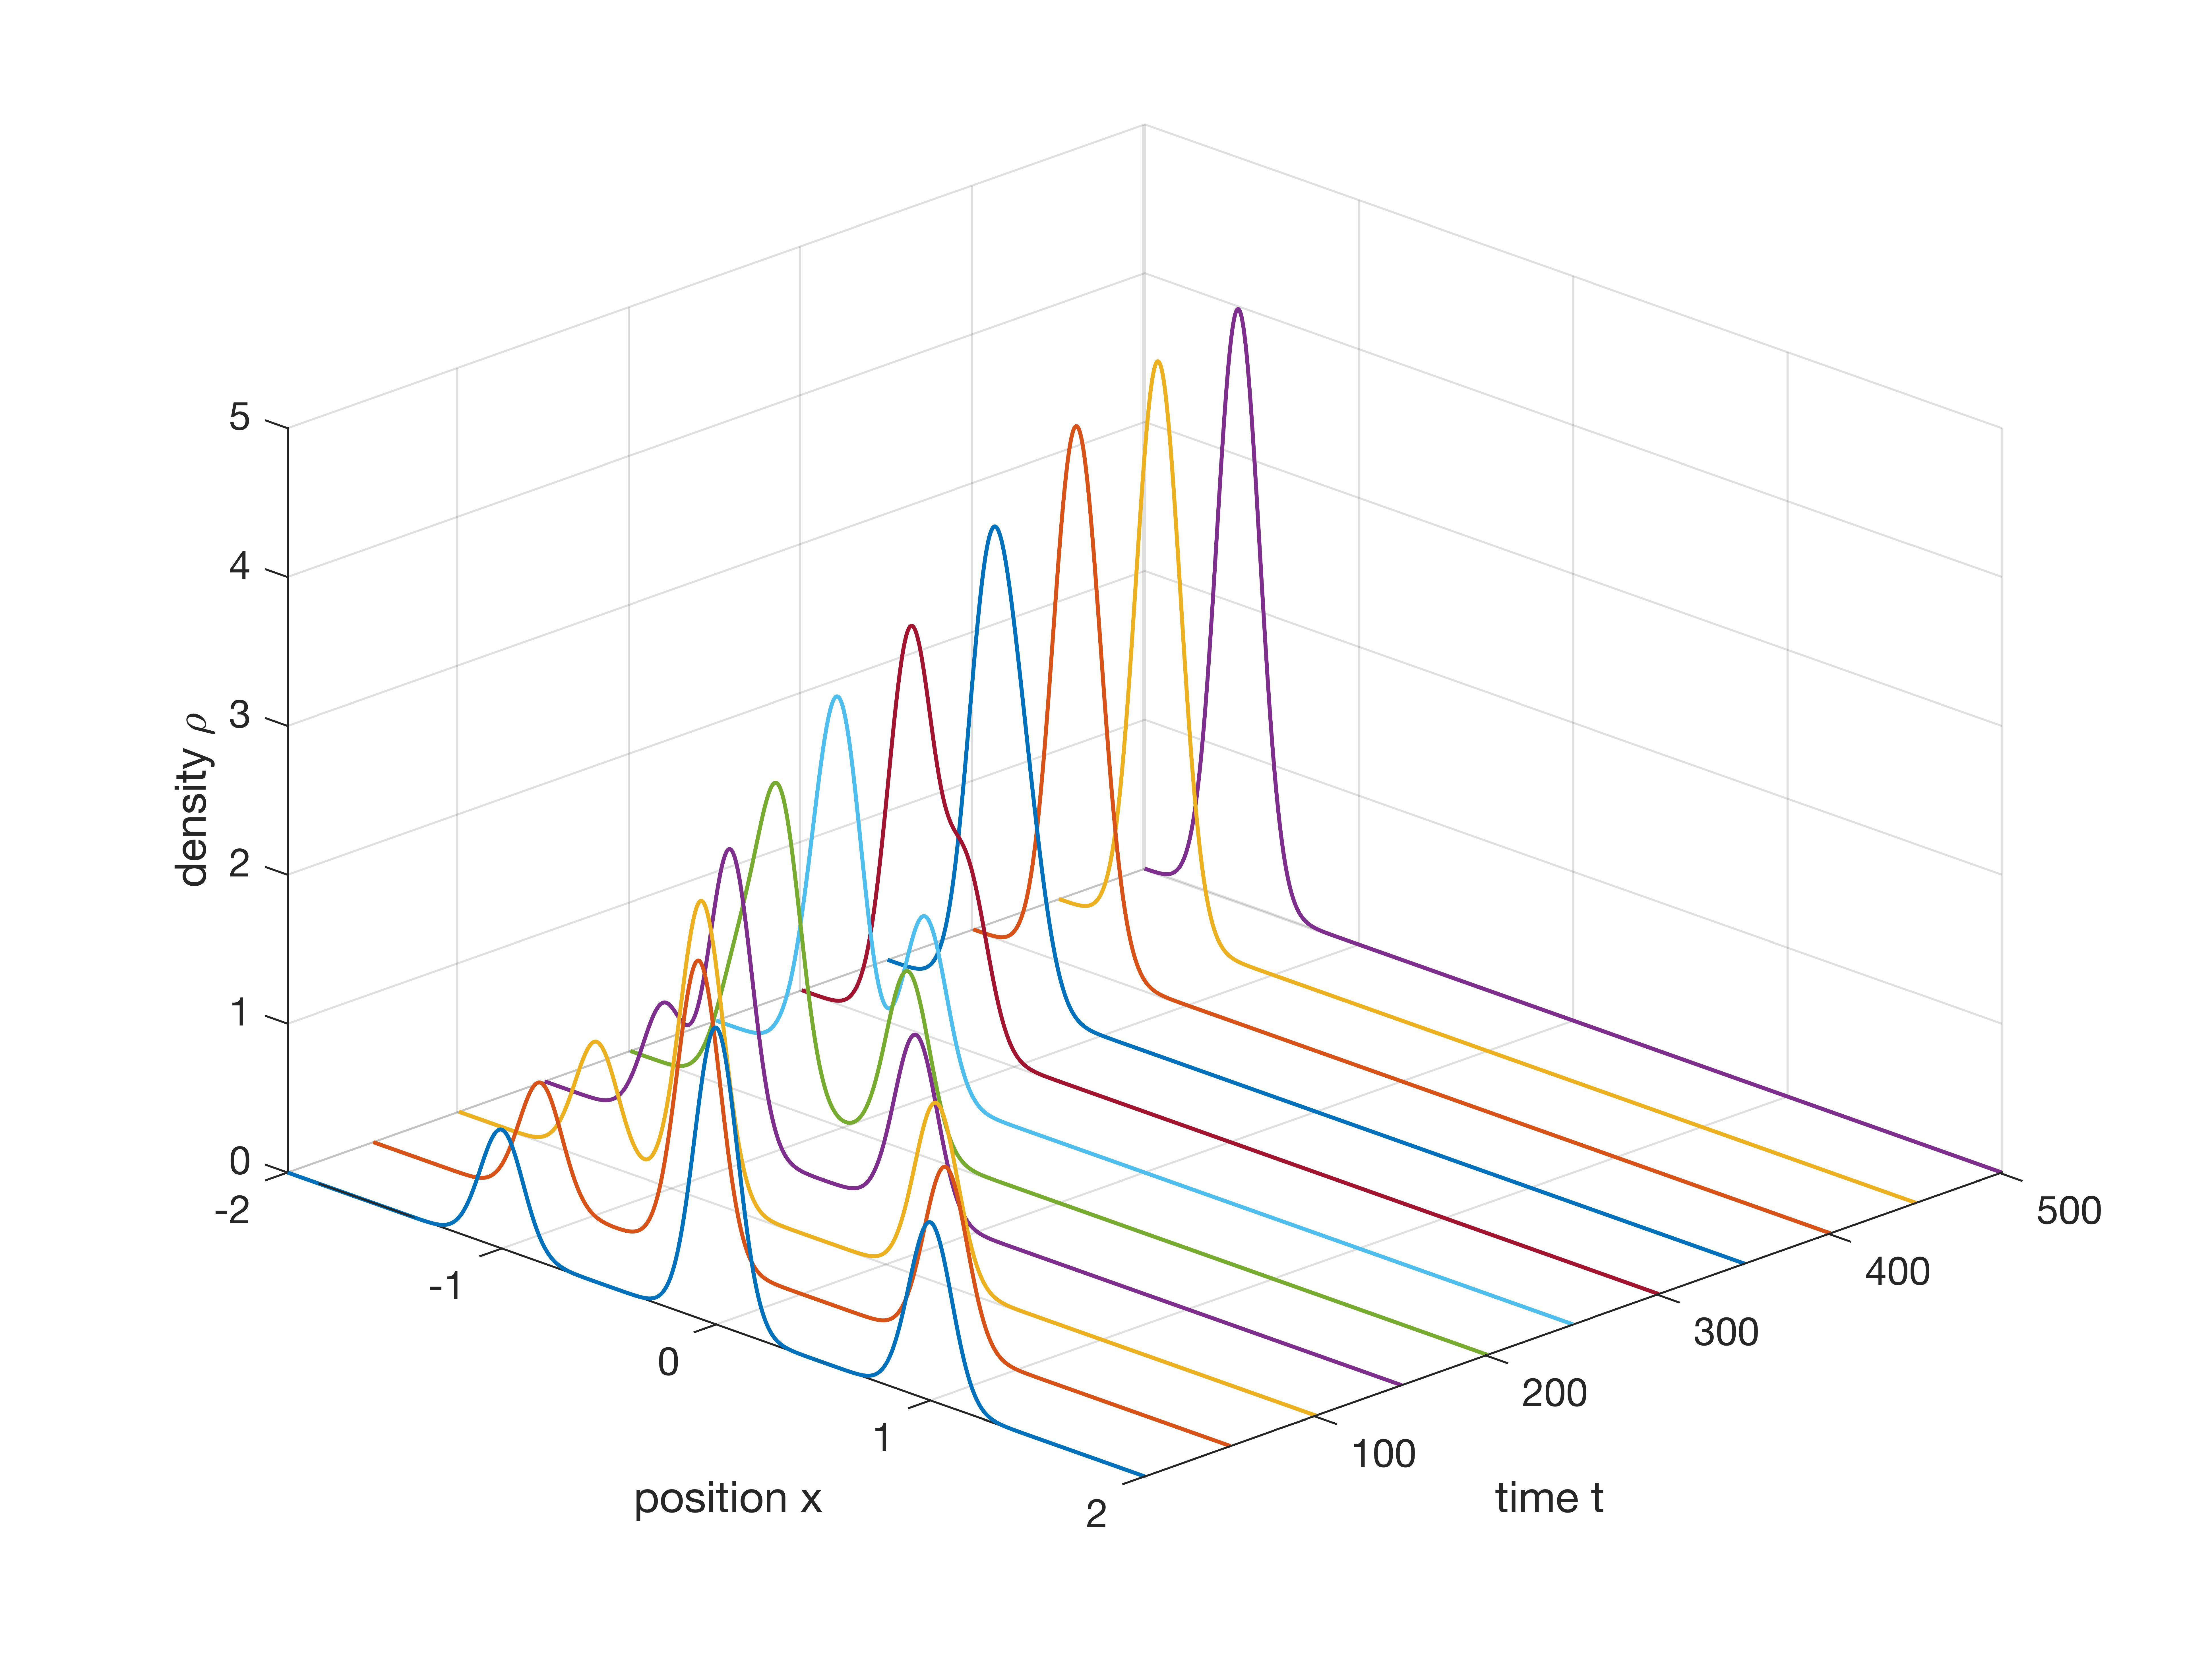
\includegraphics[width=0.7\linewidth]{degeneracy.jpg}}
  \caption{
  \scriptsize{
  This figure plots a simulation of the gradient flow associated with a potential energy functional via the discretization in an extended GMM introduced in this paper. And the time step is set as $\Delta t = 0.01$. The initial distribution is given by $\rho\lp x; 0 \rp \sim 0.2 * \mcN\lp -1, 0.1 \rp + 0.5 * \mcN\lp 0, 0.1 \rp + 0.3 * \mcN\lp 1, 0.1 \rp$. Direct calculation shows that the scaling factor $K\lp \sigma \rp \approx 2000$. The potential function is periodic as $V\lp x \rp = \sin x$. The simulation illustrates the degeneracy of extended GMMs.}}
\end{figure}
\end{frame}

\begin{frame}{Numerical experiments}
\begin{figure}[h]
  \centering
  \centerline{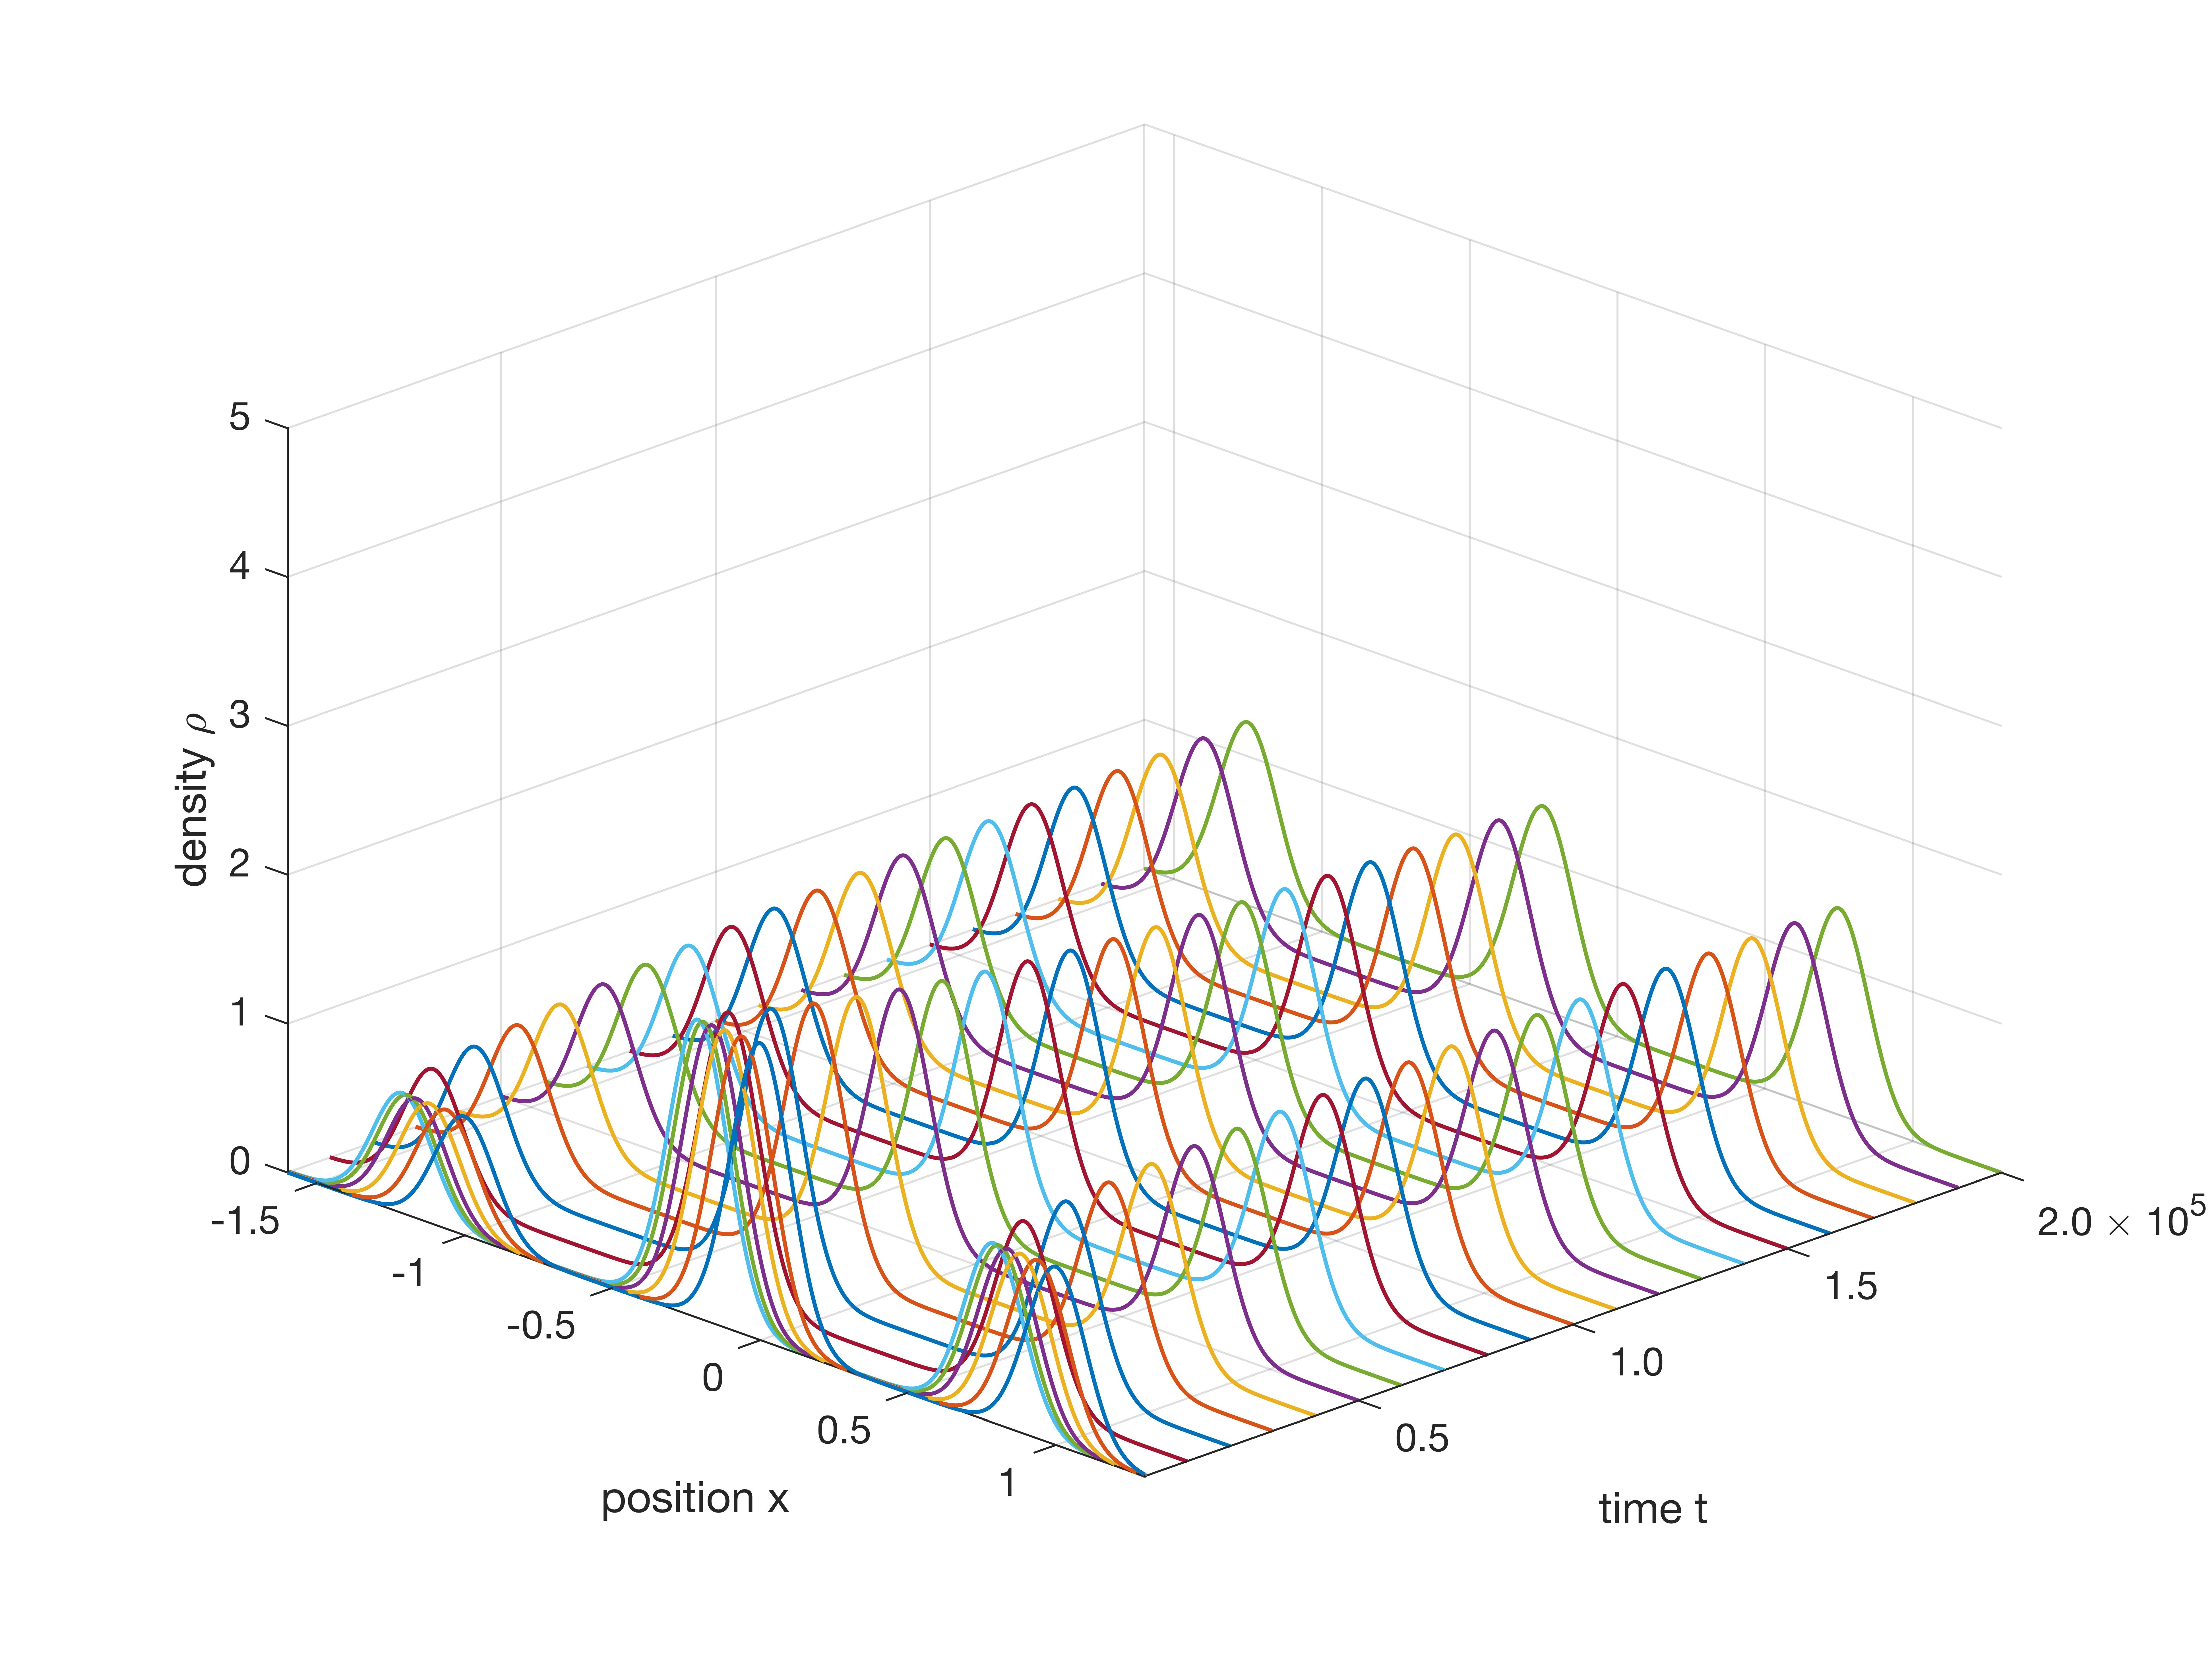
\includegraphics[width=0.6\linewidth]{mixed1.jpg}}
  \caption{
  \scriptsize{
The functional in this gradient flow is the sum of the entropy and a potential energy, i.e. $\mcE = \sum_{i = 1}^N p_i\lp \log p_i + V\lp \mu_i \rp \rp$, where the potential is periodic as $V\lp x \rp = \sin 2\pi x$. The continuous flow is drift diffusion, i.e. $\p_t \rho = \nabla \cdot \lp \rho \nabla V \rp + \Delta \rho$. And the time step is set as $\Delta t = 0.01$. The initial distribution is given by $\rho\lp x; 0 \rp \sim 0.2 * \mcN\lp -1, 0.1 \rp + 0.5 * \mcN\lp 0, 0.1 \rp + 0.3 * \mcN\lp 1, 0.1 \rp$. Consistent to our analysis, there exist two time scales in this flow: in the short scale, parameters $\mu_i$s tend to equilibrium, i.e. minimizor of $V\lp x \rp$, while in the large scale parameters $p_i$s tend to equilibrium.}}
\end{figure}
\end{frame}

\begin{frame}{Future works}
\begin{itemize}
\item 1. Consider applications in scientific computing, such as mean-field games and machine learning.
\item 2. Establish a correspondent theory for high-dimensional sample spaces.
\item 3. A complete study of the scaling Wasserstein geometry on graphs, i.e. functional inequalities, possible connection with Hamiltonian flows.
\end{itemize}
\end{frame}


\begin{frame}{Take-home message}
	\begin{itemize}
		\item 1. Scaling limits of Wasserstein GMMs exist and can be viewed as a geometric structure on graph.
		\item 2. Geometric structures on graphs further provide ways to discretize PDE preserving certain structure.
	\end{itemize}
\end{frame}


\begin{frame}{WIM and Gaussian mixture model (GMM)}
	Gaussian mixture models (GMM) are widely used in statistical inference 
	%\footnote{Huber, On Entropy Approximation for Gaussian Mixture Random Vectors, 2008} 
	(statistical models) and scientific computation. One parameterization of 1d GMM:
	%\footnote{Jianfeng Lu, Numerical methods for stochastic differential equations based on Gaussian mixture, 2018}. 
	\bequn
	\begin{aligned}
	\rho: \Theta & \rightarrow \mcP\lp \mbR \rp, \quad \Theta \subset \mbR^{N - 1},			\\
	\theta & \mapsto \rho_{\theta} = \sum_{i = 1}^{N - 1} \theta_i \lp \rho_{i + 1} - \rho_i \rp + \rho_1 = \sum_{i = 1}^{N} p_i\rho_i, \\
	1  & = \theta_0 > \theta_1 > \cdots > \theta_{N - 1} > \theta_N = 0,			\\
	\rho_i & \sim \mcN\lp \mu_i, \sigma^2 \rp, \ \mu_1 < \mu_2 < \cdots < \mu_{N - 1} < \mu_N,
	\end{aligned}
	\eequn
	We consider the pull-back metric $G_W(\theta)$ on GMM which has the following integration formula in 1d:
	\bequn
 G_W(\theta)_{ij}=\mathbb{E}_{p_\theta} \lb \frac{\lp F_{i + 1}(x;\theta) - F_{i}(x;\theta) \rp\lp F_{j + 1}(x;\theta) - F_{j}(x;\theta) \rp}{\rho(x;\theta)^2} \rb, \ F \text{ c.d.f.}
	\eequn
\end{frame}


\begin{frame}{Scaling FIM \& WIM}
\begin{itemize}
	\item Shrinking the components' variances to $0$ weakly converges to Dirac mixture model.
	\item Scaling FIM coincides with FIM on graph.
	\item Scaling WIM is diagonal and easy to be inverted.
\end{itemize}

	\begin{Thm}[Scaling FIM \& WIM]
	\scriptsize
	\bequn
		\begin{aligned}
		\lim_{\sigma \rightarrow 0} G_F\lp \theta; \sigma \rp = &\begin{pmatrix}
			\frac{1}{p_1} + \frac{1}{p_{2}} & - \frac{1}{p_2} & 0 & \cdots & 0 & 0 			\\
			- \frac{1}{p_2} & \frac{1}{p_2} + \frac{1}{p_{3}} & - \frac{1}{p_3} & \cdots & 0 & 0	\\
			0 & - \frac{1}{p_3} & \frac{1}{p_3} + \frac{1}{p_{4}} & \cdots & 0 & 0			\\
			\vdots & \vdots & \vdots & \ddots & \vdots & \vdots 						\\
			0 & 0 & 0 & \cdots & -\frac{1}{p_{N - 1}} & \frac{1}{p_{N - 1}} + \frac{1}{p_{N}}
		\end{pmatrix}		\\
		\lim_{\sigma \rightarrow 0} \frac{G_W\lp \theta; \sigma \rp}{\sqrt{2\pi^3}\frac{\sigma^3}{d}e^{\half \lp \frac{d}{2\sigma}\rp^2}} = & \begin{pmatrix}
			\frac{1}{\sqrt{p_1p_{2}}} & 0 & 0 & \cdots & 0 & 0 			\\
			0 & \frac{1}{\sqrt{p_2p_{3}}} & 0 & \cdots & 0 & 0	\\
			0 & 0 & \frac{1}{\sqrt{p_3p_{4}}} & \cdots & 0 & 0			\\
			\vdots & \vdots & \vdots & \ddots & \vdots & \vdots 						\\
			0 & 0 & 0 & \cdots & 0 & \frac{1}{\sqrt{p_{N - 1}p_{N}}}
		\end{pmatrix}.
		\end{aligned}
	\eequn
\end{Thm}
\end{frame}


\begin{frame}{Numerical experiments}
\scriptsize
	Restriction of PDE on GMM $\Longleftrightarrow$ spatial discretization of the differential operator.
	Take heat equation $\p_t \rho = \Delta \rho$ as an example, the scaling WIM provide the following spatial discretization of 2d Laplacian
	\bequn
	\begin{aligned}
	\dot{p}_{ij} = & \ - \frac{1}{d^2} \lp \sqrt{p_{i - 1,j}p_{ij}}\log \frac{p_{ij}}{p_{i - 1,j}} - \sqrt{p_{i + 1,j}p_{ij}}\log \frac{p_{i + 1,j}}{p_{ij}} \rpt			\\
	& \ \left. \qquad + \sqrt{p_{i,j - 1}p_{ij}}\log \frac{p_{ij}}{p_{i,j - 1}} - \sqrt{p_{i,j + 1}p_{ij}}\log \frac{p_{i,j + 1}}{p_{ij}} \rp.
	\end{aligned}
\eequn
\begin{figure}[h]
  \centering
  \centerline{\includegraphics[width=0.7\linewidth]{Heat_flow_2d.jpg}}
  \caption{\scriptsize{Simulation of a 2-d heat flow via discretization in this paper. The gap of the lattice and the time step are set as $d = 0.01, \Delta t = 2.5 \times 10^{-6}$ respectively. The initial distribution is given by $\rho\lp \mfx; 0 \rp = \mathbf{1}_{[-0.5, 0.5] \times [-0.5, 0.5]}\lp \mfx \rp$ and we consider its restriction to the interval $[-1, 1] \times [-1, 1]$.}}
\end{figure}
\end{frame}


\begin{frame}{Scaling WIM on extended GMM}
	Allowing mean parameters of GMM $\mu_i$s to move, one obtains WIM of the form $G_{\wtd W}^{(ext)}\lp \theta, \mu; \sigma \rp$
	\begin{Thm}[Scaling WIM for extended GMMs]
	\bequn
		\begin{aligned}
			& \lim_{\sigma \rightarrow 0}G_{\wtd W}^{(ext)}\lp \theta, \mu; \sigma \rp = \begin{pmatrix}
				\lp G_{\wtd W}^{(ext)} \rp_{\theta\theta} & \lp G_{\wtd W}^{(ext)} \rp_{\theta\mu}		\\
				\lp G_{\wtd W}^{(ext)} \rp_{\mu\theta} & \lp G_{\wtd W}^{(ext)} \rp_{\mu\mu}
			\end{pmatrix},	\\
			&  \lp G_{\wtd W}^{(ext)} \rp_{\theta\theta}, \lp G_{\wtd W}^{(ext)} \rp_{\mu\mu} \text{ both diagonal.}
		\end{aligned}
	\eequn
\end{Thm}
	The gradient flow w.r.t. a energy functional $\mcE\lp \rho \rp$ is
	\small
	\bequn\label{ext-general}
		\begin{aligned}
			\dot{\theta}_i = & \ - \frac{\sqrt{p_ip_{i + 1}}}{K\lp \sigma \rp}\lp \p_{\theta_i} \mcE\lp \rho \rp - \frac{\mu_{i + 1} - \mu_i}{2}\lp  \frac{\p_{\mu_i} \mcE\lp \rho \rp}{p_i} + \frac{\p_{\mu_{i + 1}} \mcE\lp \rho \rp}{p_{i + 1}} \rp \rp,	\\
			\dot{\mu}_i = & \ - \frac{1}{p_i}\p_{\mu_i} \mcE\lp \rho \rp + \frac{\lp \sqrt{\frac{p_{i + 1}}{p_{i}}}\frac{\mu_{i + 1} - \mu_i}{2}\p_{\theta_i} \mcE\lp \rho \rp + \sqrt{\frac{p_{i - 1}}{p_{i}}}\frac{\mu_{i} - \mu_{i - 1}}{2}\p_{\theta_{i - 1}} \mcE\lp \rho \rp \rp}{K\lp \sigma \rp},
		\end{aligned}
	\eequn
\end{frame}


\begin{frame}{Numerical experiments}
Solving PDE on extended GMM $\Longleftrightarrow$ moving mesh method. We consider solving $\p_t \rho + \nabla (\rho \nabla \sin x) = 0.$ One of the minimum is $-\frac{\pi}{2}$, where three components eventually settle down.
\begin{figure}[h]
  \centering
  \centerline{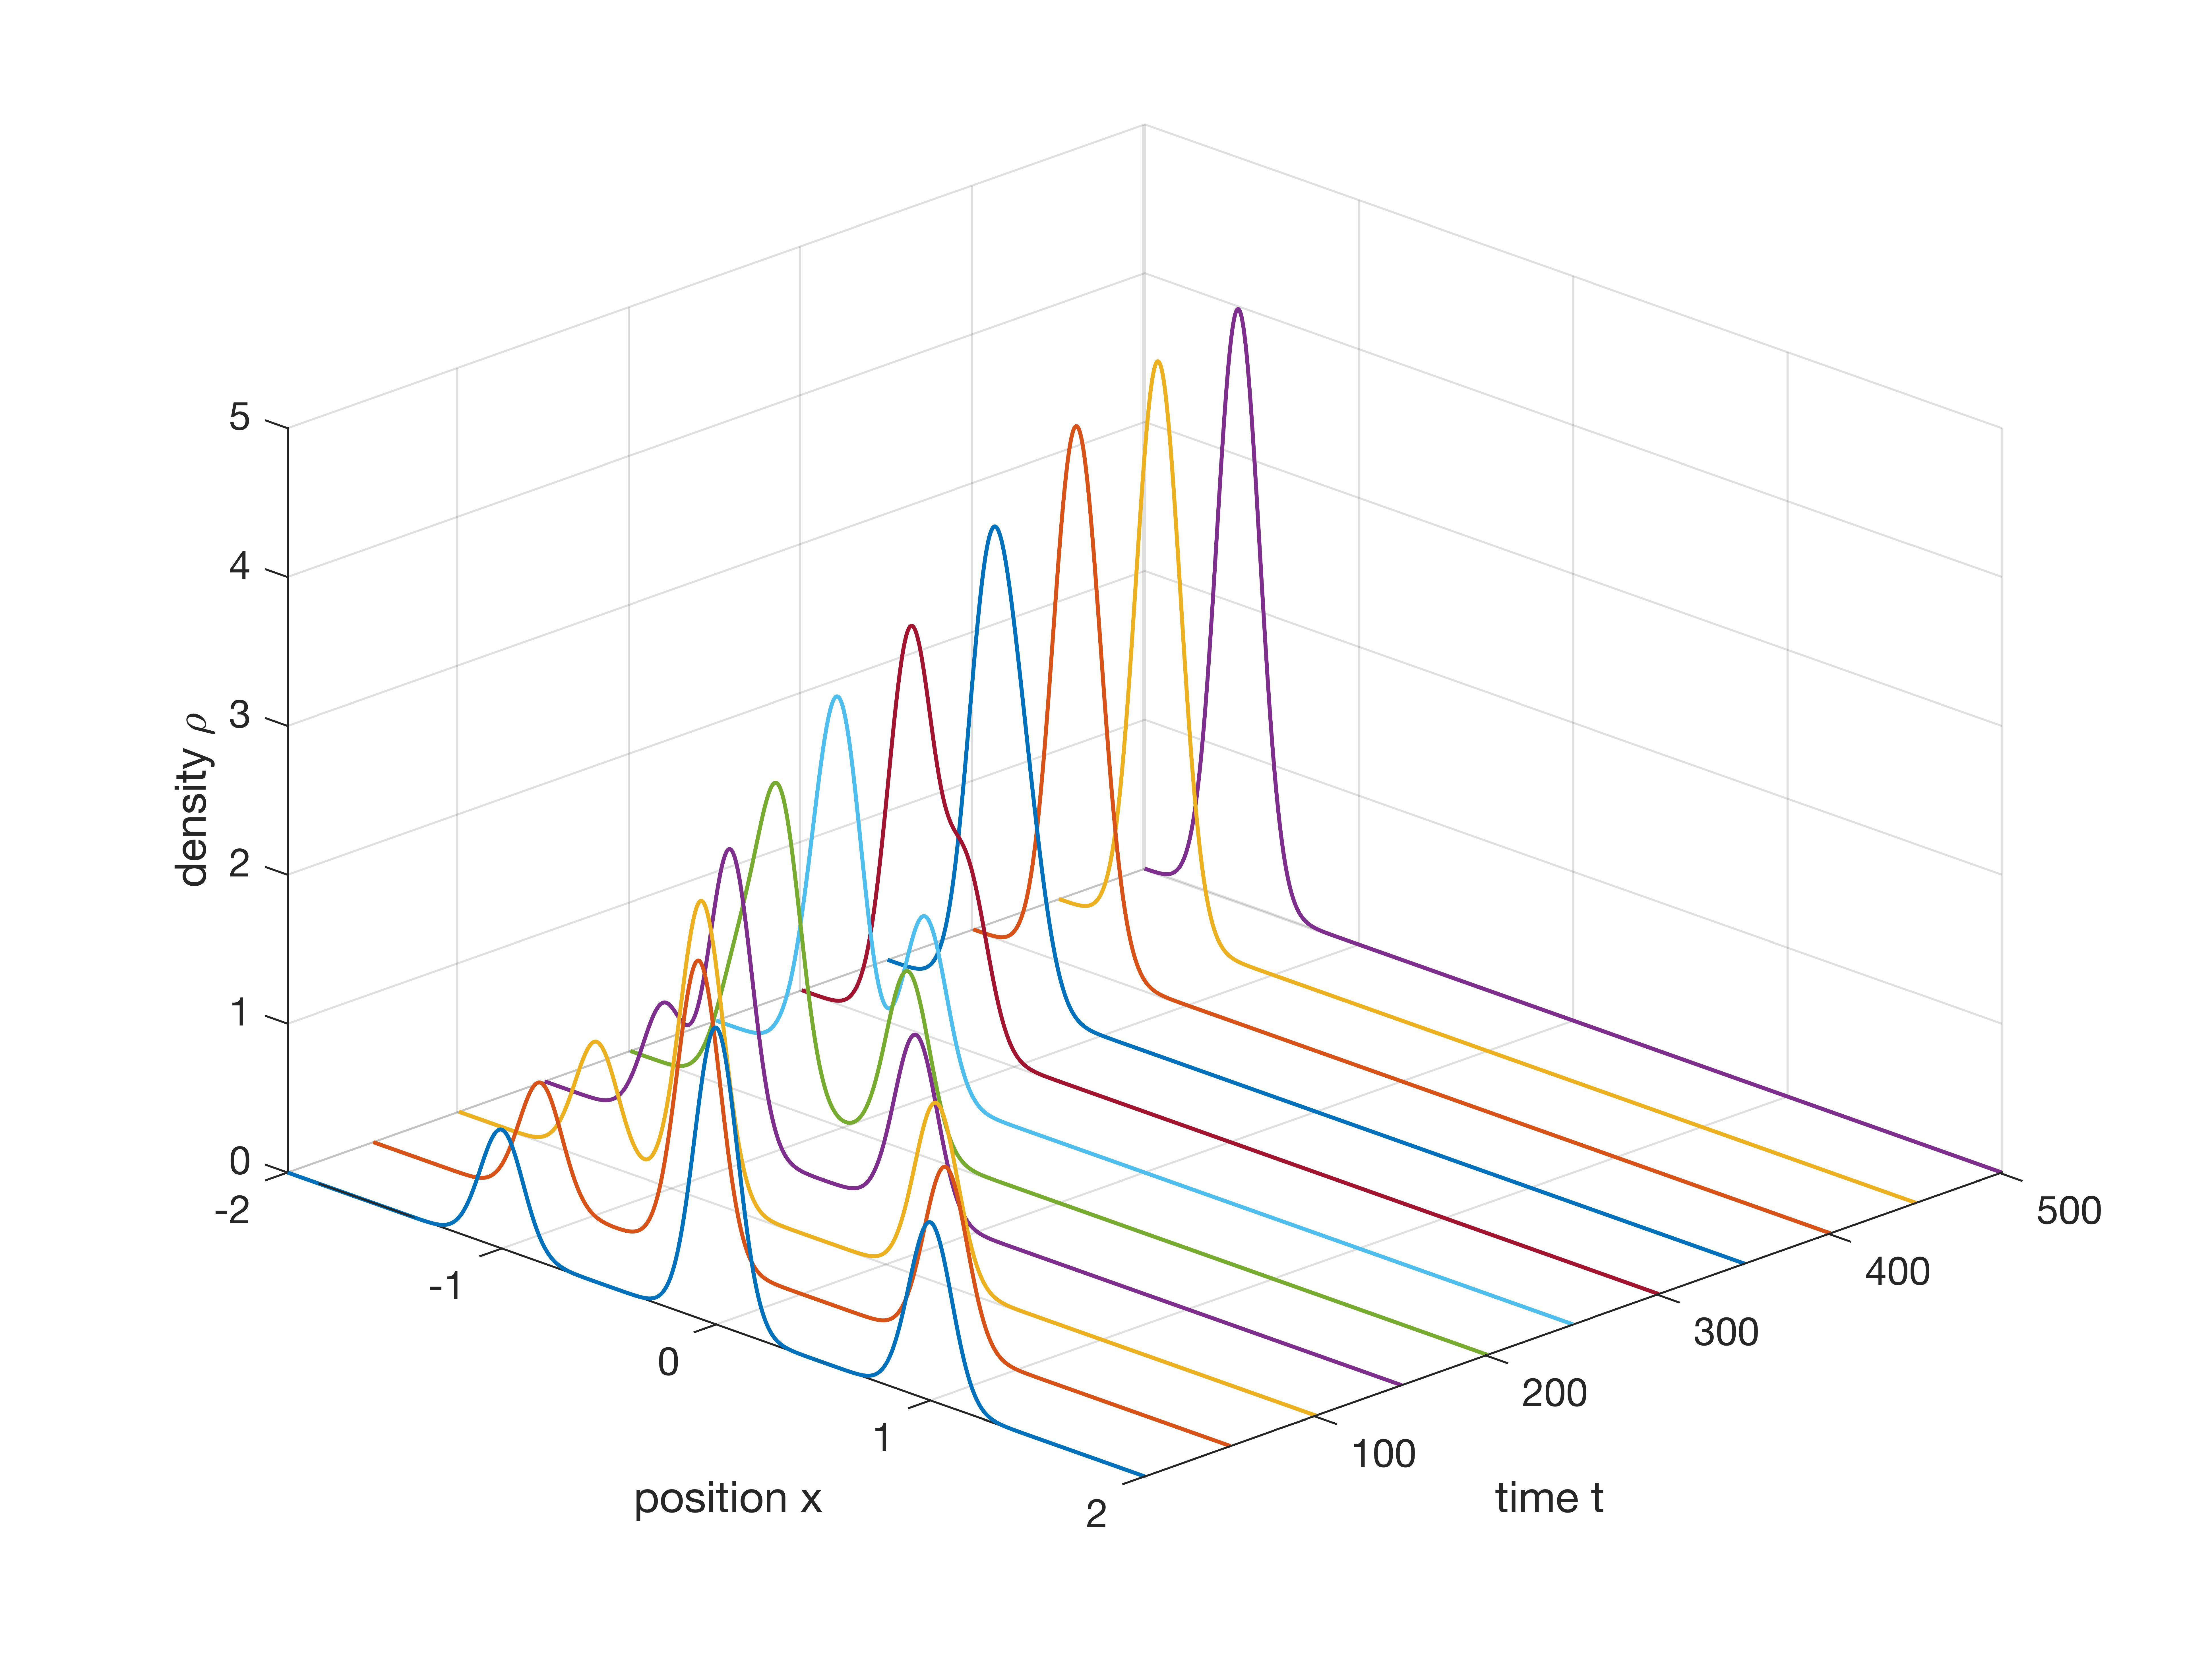
\includegraphics[width=0.7\linewidth]{degeneracy.jpg}}
  \caption{
  \scriptsize{
  This figure plots a simulation of the gradient flow associated with a potential energy functional via the discretization in an extended GMM introduced in this paper. And the time step is set as $\Delta t = 0.01$. The initial distribution is given by $\rho\lp x; 0 \rp \sim 0.2 * \mcN\lp -1, 0.1 \rp + 0.5 * \mcN\lp 0, 0.1 \rp + 0.3 * \mcN\lp 1, 0.1 \rp$. Direct calculation shows that the scaling factor $K\lp \sigma \rp \approx 2000$. The potential function is periodic as $V\lp x \rp = \sin x$. The simulation illustrates the degeneracy of extended GMMs.}}
\end{figure}
\end{frame}


\end{document}